\documentclass{article}
\usepackage[utf8]{inputenc}
\setlength{\parindent}{0em}
\setlength{\parskip}{3 mm}
\usepackage{amsmath}
\usepackage{natbib}
\bibliographystyle{abbrvnat}
\setcitestyle{authoryear,open={(},close={)}}
\usepackage{graphicx}
\DeclareRobustCommand{\firstsecond}[2]{#1}
\usepackage{float}
\usepackage{url}
\usepackage{lipsum}
\usepackage{xcolor}
\usepackage{caption}
\usepackage{subcaption}
\usepackage{booktabs}
\usepackage[margin=1in]{geometry}
\newcommand{\E}{\mathrm{E}}
\newcommand{\Var}{\mathrm{Var}}
\newcommand{\Cov}{\mathrm{Cov}}

\title{A `Ghetto' of One's Own: \\
Communal Violence, Residential Segregation and Group Education Outcomes in India}
\author{Aarushi Kalra\thanks{Economics, Brown University. I am grateful to Andrew Foster, Bryce Steinberg, Jesse Shapiro, Patrick Heller, John Friedman, David Weil, Jesse Bruhn, Alisa Tazhitdinova, Daniel Bjorkegren, Stelios Michalopoulos, Martin Mattsson, Naveen Bharathi, Diane Coffey and seminar participants at Brown University for invaluable comments. I thank Naman Garg, Jose Belmar, Marcela Mello, Joao Garcia, Giulia Buccione, Aastha Tyagi, Suvaid Yaseen, Harkirat Singh, Saket Tiwari, Bhanu Joshi, and Sagar Wadhwa for their support. All remaining errors are my own.}}
\date{February 2021}

\begin{document}

\maketitle

\begin{abstract}
    \noindent How does ethnic violence and subsequent segregation shape children's lives? Using exogenous variation in communal violence due to a Hindu nationalist campaign tour across Indian states, I show that ethnic violence displaces Muslims to segregated neighbourhoods. Surprisingly, I find that post-event primary education levels are higher for Muslims in cities that were more susceptible to rioting. This is on account of increased residential segregation and greater spatial cohesion within communities threatened by violence. Under reasonable assumptions on the direction of bias, instrumental variable estimates predict that Muslims are 5 percent more likely to attain primary education with a 10 percentage point increase in segregation. This narrows the gaps in early education between Muslims and non-Muslims.
\end{abstract}

\newpage
\section{Introduction}
Inter-group inequality has serious economic ramifications. For instance, \cite{alesina2016ethnic} document strong negative association between ethnic inequality and GDP per capita across Africa. Analyzing inter-group inequality is especially significant in the case of India which has witnessed a heightened role of ethnic and religious identity in expressions of conflict as well as inequality. Despite recent poverty reductions, Indian Muslims earn less than Hindu Dalits\footnote{The preferred political term for people belonging to the lowest caste in India, characterised as "untouchable": \url{https://en.wikipedia.org/wiki/Dalit}.}, which is counted among the most historically disadvantaged communities in India. Muslim per capita income represents 68\% Dalit per capita income in Haryana, 69\% in Gujarat, and 87\% in Maharashtra (NSSO, 2012). Furthermore, only 14\% of the Muslim population in India was likely to complete college education in 2018 \citep{kalai.2019}. 

My work investigates how inter-group conflict impacts relative education outcomes of Muslims. Communal conflict not only exacerbates between-group income disparities \citep{esteban2011linking}, it also leads to discriminatory practices and policies against the dominated group. This paper gauges education choices that members of a threatened community (in this case, Muslims) make in the aftermath of violence over the long run. This is done using plausibly exogenous variation in communal violence due to a Hindu nationalist campaign tour across Indian states. 

I find that ethnic violence is associated with \textit{improvement} in education outcomes of Muslims children in India. I take note of narrower education gap between Muslims and non-Muslims (as measured in various rounds of the NSS Employment-Unemployment Surveys between 1987 and 2012) in geographies with a history of Hindu-Muslim conflict\footnote{This is important because inter-group inequality and inter-generational economic mobility in India is best measured using data on education attainment \citep{asher.2018}, in the presence of measurement error in income data collected using survey methods.}. I provide descriptive evidence that stronger social ties consequenced by violence, may be driving this very surprising result. In lieu of micro-measures for within-community ties, I show high degree of association between cities segregated along religious lines, and cities with a history of communal tensions.

Identifying causal impact of communal violence is difficult because riots are more likely to occur in areas with rising Muslim incomes \citep{mitra.2014}. This is likely to generate omitted variable bias in the OLS relationship between communal riots and education outcomes due to selection. To overcome this challenge, I leverage plausibly exogenous variation in riots that emerges from the planned path of a series of anti-Muslim campaign events. Known as the \textit{Ram Rath Yatra} (henceforth, \emph{Yatra}), this controversial campaign trail across several Indian states\footnote{Figure \ref{fig:route_p} shows the planned route of the campaign trail.}, was organized by the Bhartiya Janata Party (henceforth, BJP) in 1990. During this campaign, many prominent leaders of the BJP planned to travel 10,000 kilometres \citep{mishra.2015} to mobilize support for the demolition of a 16$^{th}$ century Mosque in India\footnote{The campaign commenced at the site of a famous temple in Somnath (Gujarat), and was to conclude in Ayodhya, the \emph{purported} site of another temple allegedly destroyed by Mughal rulers.}. This led to communal riots, majority of which took place on or very close to the campaign route \citep{engineer1991bloody}.

\begin{figure}[h!]
    \centering
    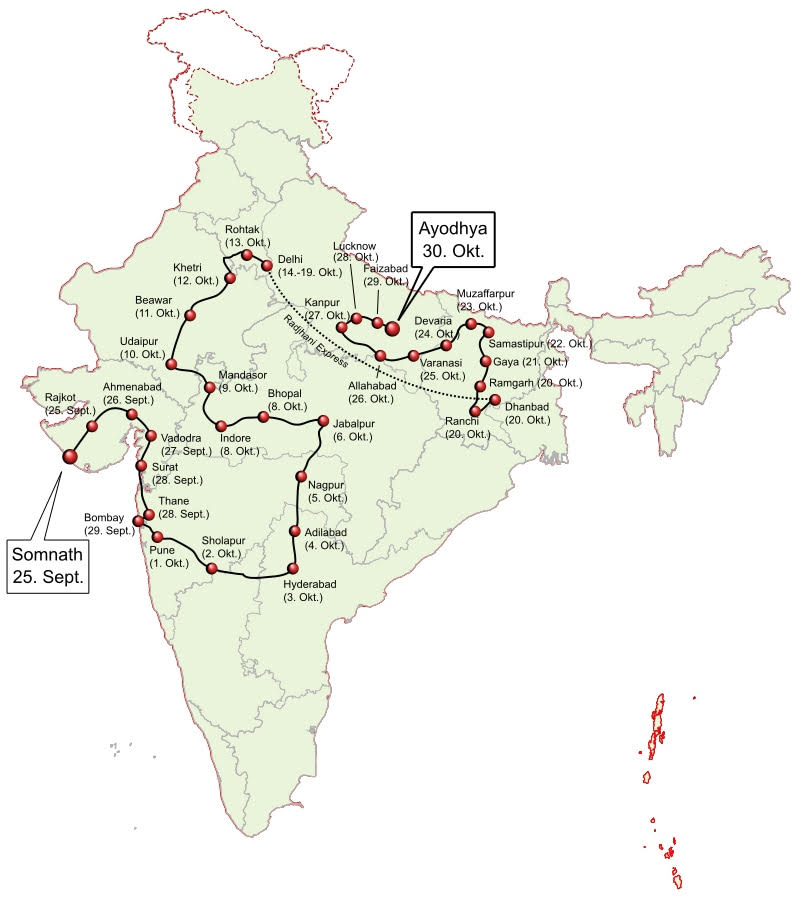
\includegraphics[scale=0.3]{images/plan_route.jpg}
    \caption{Plan of \emph{Rath Yatra} Campaign Route, \emph{Rath Yatra} (Source: David Ludden, \emph{India and South Asia: A Short History}).}
    \label{fig:route_p}
\end{figure}

I find that Muslim cohorts starting school after the event in 1990 attain lower levels of primary education, relative to non-Muslims, in cities farther away from the campaign route (that were less susceptible to rioting). In particular, for Muslims in cohorts born between 1981-85, the probability of attaining primary education fell by 0.24\%, and by 0.23\% for Muslims in cohort born between 1986-90, with every 10 kilometres away from the campaign route. 

I construct placebo tests by using difference in the planned and actual route of the \emph{Yatra}. I claim that exposure to \emph{Yatra} was exogenously determined, by assuming that the location of obstruction in the route is independent of outcome variables. This is granted by an unexpected impediment in the path of the campaign, when the leader of the movement (LK Advani) was arrested in the state of Bihar, before entering the destination state of Uttar Pradesh\footnote{See Section \ref{data_yatra} for background details.}. The placebo tests are successful, as these results do not hold with respect to the planned \textit{Yatra} route in places where the campaign could not enter.

I demonstrate that \textit{Yatra} provides quasi-random variation in communal violence, as I do not find differential trends in the distribution of Muslim consumption expenditures, or in education infrastructure, pre and post-\textit{Yatra}, in cities along the campaign route. While I show balance in education infrastructure as a function of the continuous treatment, I cannot rule out that the campaign was more likely to go to more populous cities. Therefore, I measure the effect of being closer to the \textit{Yatra} route among cities with similar observable characteristics. I estimate the effect of violence on education by matching propensity scores with continuous treatment \citep{hirano2004propensity}. The treatment effect on early education remains statistically significant and negative for cohorts starting school after 1990. 

I develop a theory of residential segregation as a channel of improved early education outcomes among Muslims following \cite{abdulkadirouglu2014elite}, and impose weak assumptions on the direction of bias induced by other unobserved factors. I demonstrate that neighbourhood effects on Muslim education outcomes are positive, when unobservable factors in the model are argued to impact Muslim education outcomes negatively. I then build causal estimates of neighbourhood effects on early education outcomes of Muslims. 
%However, the violence directly manifests itself as poorer education outcomes for cohorts that were growing up at the time of violence (for cohorts born between 1971 and 1980), and were living in cities closer to the \emph{Yatra} route. This may impact education attainment of cohorts born after 1980, via the channel of parental education levels. Note that this can be expected to lower Muslim education attainment, whereas neighbourhood effects are shown to go in the opposite direction.

I find a positive correlation between riots and residential segregation. Not only do I find a negative relationship between riots and distance from the \emph{Yatra}, I also find a strong and negative relationship between residential segregation and \textit{Yatra} in States that the campaign entered. That is, the dissimilarity index in 2013 falls by 0.2\% with every 10 kilometres away from the route.  

I check if this correlation is spurious, by looking for treatment effects on `untreated' groups. Displacement on account of communal riots between Hindus and Muslims should not affect residential patterns of the Scheduled Caste (henceforth, SC) population, who have also been documented to live in segregated neighbourhoods in Indian cities \citep{bharathi2018isolated} and are being thought of as the untreated group. And indeed, I am able to demonstrate that the continuous treatment, by way of distance from the \textit{Yatra} route, is uncorrelated with segregation of SC populations. The placebo test is successful in this regard as well, because the relationship between segregation and planned \textit{Yatra} is diametrically opposed to my findings for treated cities. I also check for treatment effects in states that were not exposed to the campaign (controlling for spillovers), and do not find any correlation of the treatment with segregation of Muslims in these states.  

Finally, I offer a discussion of possible channels that may be driving the surprising effect of communal violence and segregation on Muslim education outcomes. I hypothesize that \textit{strong ties} \citep{granovetter1973strength} within a community provide role models and resources to pursue primary education, while the absence of \textit{weak ties} hinders representation of Muslims in colleges and Universities. Targeted violence may strengthen already existing links, in order to rebuild businesses and incomes that were lost due to the rioting. This  hypothesis  is  supported by qualitative evidence in \cite{jaffrelot2012muslims}, which claims that members of Muslim enclaves, segregated by communal violence in Gujarat, eventually achieved higher socio-economic status, despite the conspicuously absent public provision of welfare for this community. This is because communities are very tightly knit in the aftermath of violence, as members support each other to rebuild businesses and incomes. 

This paper speaks to four strands of literature in Economics: one deals with measurement, causes and effects of ethnic or inter-group inequality; while the other relates to the role of ethnic violence in determining socio-economic outcomes. In interrogating channels through which inter-group violence impacts education outcomes, my work is, thirdly, related to literature investigating the relationship between residential segregation of historically disadvantaged groups and their economic outcomes. Finally, this paper picks up on the recent literature on human capital formation among Muslim communities.

First, this paper extends the vast and rapidly growing literature on inter-group inequality and inter-generational economic mobility \citep{chetty2014land} to developing countries. \cite{alesina2016ethnic} measure consequences of ethnic inequality across African countries, whereas \cite{sethi2010group} investigate the relationship between group identities and mobility for the Scheduled Castes and Scheduled Tribes in India. In particular, my work is especially relevant in contexts where religion is key in the process of identity formation, and is closely tied with the work of \cite{alesina2020religion} and \cite{asher.2018}, who study the relationship of Muslim identity with educational mobility in Africa and India, respectively. This paper contributes to this literature by investigating the causes for differences in educational attainment across religious groups, and the role of conflict herein.  

Second, this work fits into the literature on the economics of ethnic conflict. \cite{mitra.2014} interrogate the correlates of communal riots and verify the hypothesis that a relative increase in Muslim income or consumption is associated with an increase in the probability of a riot. \cite{iyer2015religious} as well as \cite{blakeslee.2018} use Instrumental Variable approaches to show that Hindu-Muslim riots increase the vote share of the BJP in elections that follow such rioting. I borrow Blakeslee's (2018) assignment of electoral wards to the \emph{Yatra} route (in Figure \ref{fig:route_b}) to construct my continuous treatment, i.e. distance of a city from the \textit{Yatra} route. \cite{field2008segregation} consider the case of communal violence in Ahemdabad (Gujarat), and find that riots were more likely to break out in more integrated neighbourhoods. They also hypothesized, albeit did not test, that residential segregation was likely to increase after the riots. I bring evidence to test this hypothesis, while looking at the impact of violence on a broader range of outcome variables.  

\begin{figure}[h!]
    \centering
    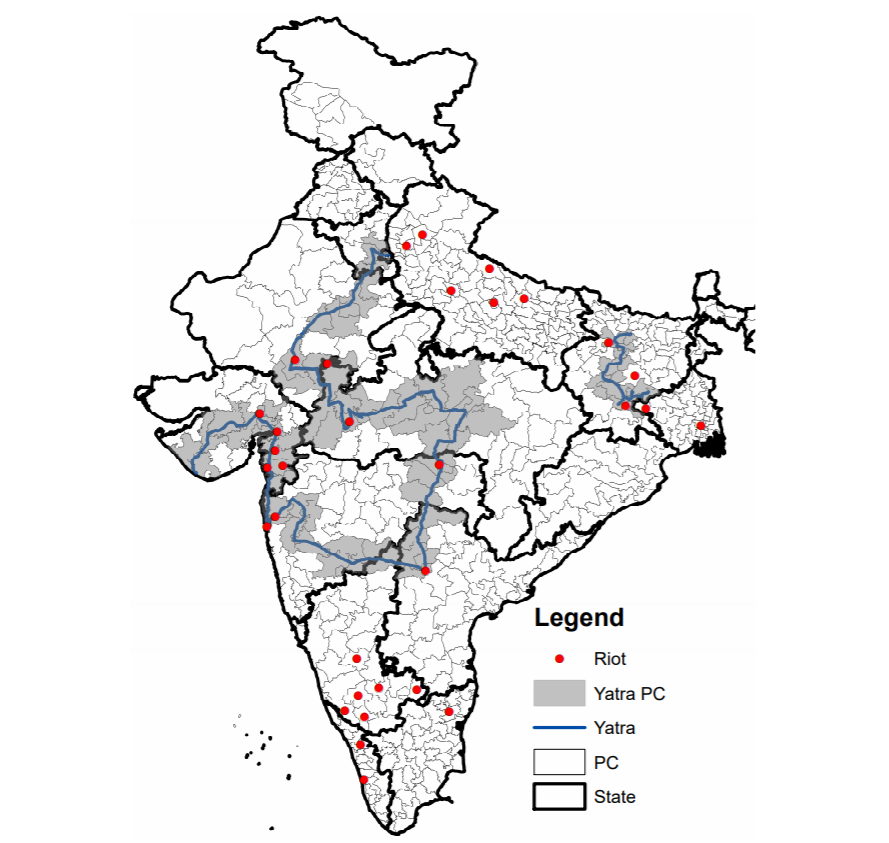
\includegraphics[scale=0.55]{images/blakeslee.png}
    \caption{Actual campaign route, \emph{Rath Yatra} (Source: \cite{blakeslee.2018})}
    \label{fig:route_b}
\end{figure}

Third, this analysis deals with the literature on residential segregation and socio-economic outcomes of marginalized groups in the Indian context. \cite{chetty2018impacts} analyze the effect of neighbourhoods on child development across races in the US. This is done, in part, by exploiting exogenous displacement shocks, and therefore, ties very closely with my empirical strategy. \cite{susewind2017muslims} provides a description of segregation across religious lines in India using electorate rolls at the ward level for 11 cities\footnote{A ward is a local administrative unit of a city, with an average population of 1,500 to 6,000 for small statutory towns, and 30,000 to 200,000 for larger metropolitan cities \citep{prasad2006wards}. It is therefore, much larger than an enumeration block (which measures a neighbourhood in this paper) with population of 650 to 700 \citep{secc.2011}.}. However, \cite{bharathi2018isolated} demonstrates that ward level variation does not fully capture concentration of social groups in various parts of a city, and therefore, document segregation along caste lines at neighbourhood levels.

The literature on residential segregation in India has mainly focused on segregation along caste, and not religious lines\footnote{This is primarily due to the fact that most government sources of data do not share information at the neighbourhood level, to ensure safety of historically marginalised groups. Neighbourhood level data (electoral rolls, for instance) on Muslims is documented to make the community more vulnerable in the event of a riot \citep{jaffrelot2012muslims}.}. Most recently, \cite{adukia.2018} use neighbourhood and religious identifiers in the Economic Census to provide descriptive evidence of residential segregation along communal lines. Mine is the first attempt to provide causal estimates of neighbourhood effects on long-term education outcomes among Muslims. 

Finally, there is sprouting interest in the positive effects of ethnic enclaves in Developing Countries. Despite lower wealth, consumption, educational attainment, and access to state services \citep{kalai.2019}, Muslims exhibit higher human capital accumulation in early childhood \citep{bhalotra2010puzzle}. \cite{geruso2018neighborhood} link religious composition of neighbourhoods with lower infant mortality among Muslims, through the channel of sanitation. \cite{meyersson2014islamic} shows that women's political participation as well as secular high school education rates increased in Turkish municipalities where Islamic parties came to power, due to strong within-community ties. This paper links segregated Muslim enclaves with higher early education attainment for Muslims in India.

The rest of the paper is organized as follows: Section \ref{data} describes the data sources along with a brief background of the \textit{Yatra}, Section \ref{empirical_strategy} describes the Empirical Strategy, Section \ref{results} describes the results from the IV estimation, Section \ref{placebo} demonstrates a range of robustness checks, Section \ref{discussion} discusses the results along with necessary caveats and concludes. 

\section{Data}\label{data}
In this section, I set the socio-political context and provide a broad overview of the background in which I operate. I also provide a detailed description of the employed data sources. 

\subsection{\textit{Ram Rath Yatra} Route} \label{data_yatra}
\textbf{Background}

The \emph{Ram Rath Yatra} rally was part of the \emph{Ram Janmabhoomi} (`birthplace of \emph{Ram}') movement. The goal of this movement was the construction of a temple for the mythical king \emph{Ram} at his legendary birthplace in Ayodhaya, Uttar Pradesh\footnote{This goal was achieved on August 5, 2020 when Prime Minister Narendra Modi laid the foundation stone of the \emph{Ram} Temple after a long legal battle. \url{https://www.bbc.com/news/world-asia-india-53577942}.}. According to supporters of this campaign, the original temple at his birthplace was destroyed by the Mughal ruler Babur, who in its place built a mosque, \emph{Babri Masjid} in 1527 \citep{ramjanmabhoomi}. These claims are made based on archaeological evidence that has been challenged by independent historians and archaeologists \citep{gopal1990political}.

This movement gained importance on the Indian political landscape due to various factors including,

\begin{itemize}
\item The breaking out of an armed rebellion against the Indian state in Muslim-majority region of Kashmir, claiming more than tens of thousands of lives\footnote{\url{https://www.bbc.com/news/10537286}.}

\item The Mandal Commission award of affirmative action to backward castes threatened the position of upper-caste Hindus \citep{balagopal1990anti}. In 1980, the Socially and Economically Backward Classes Commission's report recommended that members of Other Backward Classes (OBC) be granted reservations in 27\% of jobs under public sector undertakings

\item The Shah Bano case in the Supreme Court of India, which was a controversial maintenance lawsuit where the Supreme Court delivered a judgment favouring maintenance given to an aggrieved divorced Muslim woman. The Congress government enacted a law, shifting the onus of maintaining her to her relatives or the Waqf Board, solidifying the perception that the Congress party favoured Muslims \citep{pathak1989shahbano}
\end{itemize}

These political factors culminated into hostility between the two communities, and led to Hindus feeling threatened in a country where they constitute the majority population. The objective of the campaign was to promote a unitary Hindu identity transcending the divisive caste system. This identity was perceived to be threatened on account of the Muslim community and upward mobility of backward castes \citep{jaffrelot2010religion}. 

The \emph{Yatra} commenced on September 25, 1990, in the state of Gujarat. Political rallies and religious processions were held along the path of the route, with Hindu activists greeting and cheering the campaign wherever it went\footnote{In his film \emph{In the name of God}, director Anand Patwardhan captured the site of thousands of people assembling to welcome the arrival of the \emph{Yatra} in various cities, thus deeply polarizing the political environment.}. 

\textbf{The Route}

\cite{blakeslee.2018} constructed data on the route of the \emph{Yatra} using daily accounts from the \emph{The Times of India}, one of the major national newspapers in India. Using these journalistic accounts along with GIS maps of Parliamentary constituencies, the road network and built-up areas, he determines the constituencies through which the \emph{Yatra} had actually passed.

I use Figure \ref{fig:route_b} to plot the \emph{Yatra} route on GIS maps and then compute the distance of the route from sample cities, in kilometres. This is done for the states through which the \emph{Yatra} was planned to go: namely Gujarat, Maharashtra, Andhra Pradesh, Madhya Pradesh, Rajasthan, Haryana, Bihar and Uttar Pradesh. 

Note that the route does not enter Uttar Pradesh (UP), whereas Ayodhya (the destination of the route) is in UP. This was on account of Bihar government's decision to arrest LK Advani, the leader of this campaign, before they entered UP\footnote{On October 23, LK Advani, one of the most powerful leaders of the BJP who led the \emph{Yatra}, was arrested in Bihar's Samastipur district on the orders of then Chief Minister Lalu Yadav to prevent him from proceeding to Ayodhya.}. This is key for my identification strategy as I calibrate distance of a city in UP from \emph{planned} route, using Figure \ref{fig:route_p} and GIS maps, to perform robustness checks.   

\subsection{Riots}
A number of Hindu-Muslim riots erupted along the route of the \emph{Yatra}. On November 1, 1990 (a day after the planned culmination of \emph{Yatra}), riots broke out in a number of places, and curfew was enacted in at least 30 districts \citep{engineer1991bloody}. Of the 64 Hindu Muslim riots which took place between 1990-91, 35 occurred during the 6 weeks surrounding the \emph{Yatra}, 11 of which were in constituencies through which it passed \citep{blakeslee.2018}. 

In Figure \ref{fig:riots_yatra}, I use \cite{vw.2006} dataset on communal violence in India, to plot the count of riots (in the aftermath of the \textit{Yatra}) as function of distance from \textit{Yatra} route. This data set provides comprehensive information on all Hindu-Muslim riots reported in a newspaper of record (\textit{The Times of India}, Bombay edition), from January 1950 through December 1995. The data consists of information about the location as well as injuries and deaths. Of particular interest are the riots between 1990 (start of the \emph{Yatra} campaign) until 1993 (after the ultimate demolition of Babri Masjid in December 1992).

\begin{figure}[H]
    \centering
    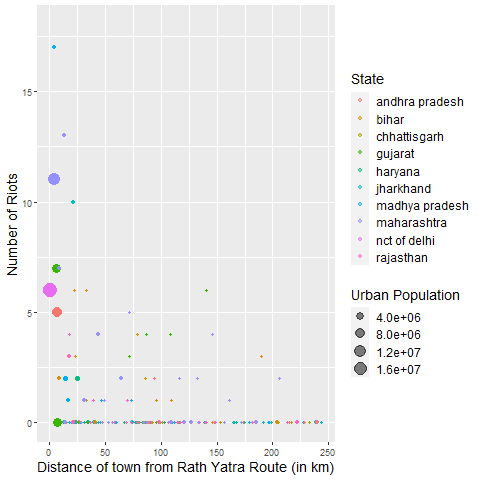
\includegraphics[scale = 0.6]{images/graph_riots_yatra.png}
    \caption{Number of Riots (1990-93) by Distance from \textit{Yatra} route}
    \label{fig:riots_yatra}
\end{figure}

I geocode this data\footnote{courtesy, Naman Garg for geocoding cities in \cite{vw.2006}.} to match with town level indices constructed using the Economic and Population Censuses and \cite{sedac}. 

\subsection{Education Outcomes}
I access demographic information of individuals in sample households--level of education, gender and age-- from the National Sample Survey Organization's Employment Unemployment Surveys (NSS-EUS, thick rounds between 43 \citep{eus.1988} to 68 \citep{eus.2012}). I obtain household level attributes like religion, social group, and consumption level from the same data source. I normalize current consumption and wages (in Rupees), setting 1983 as the base year, using disinflation factors from Consumer Price Index for Industrial Workers series \citep{cpi_iw}.

I link urban centres of districts in the NSS data with cities in the Economic and Population Censuses, and use district urban averages as proxies for city-level averages, following \cite{greenstone2014environmental}. Furthermore, since district boundaries have changed over time \citep{somanathan2009mapping}, I use district keys from NSS-EUS round 43, held in 1987\footnote{courtesy Bryce Steinberg, for sharing district mappings across NSS rounds} to harmonize administrative boundaries over the sample period \footnote{The resulting imprecision in matching leads to considerable noise. See \cite{harari2020cities} for a detailed treatment of matching Indian cities in Census and NSS data}.

I divide the sample of Muslim and Non-Muslim males (after dropping members of Scheduled Castes (SC) and Scheduled Tribes (STs)) into six cohorts: (1) Born before 1950, (2) Born 1951-60, (3) Born 1961-70, (4) Born 1971-80, (5) Born 1981-90 and (6) Born between 1991-96. Figure \ref{fig:within_group} shows trends in educational attainment within the two groups of interest: Muslims and Non-Muslims. %I only consider the sample of males as cultural factors (unrelated to moving on account of riots) may have impacted trends in educational attainment for Muslim and Non-Muslim women differentially \citep{ghosh1997changing}. 

\begin{figure}[H]
    \centering
    \begin{subfigure}{.49\textwidth}
        \centering
        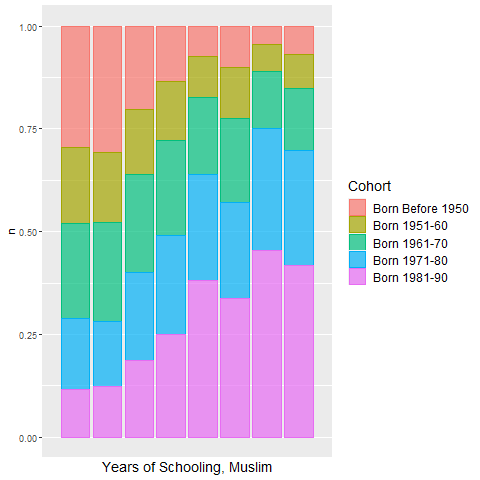
\includegraphics[width = \textwidth]{images/graph_edu_mus.png}
    \end{subfigure}
    \begin{subfigure}{.49\textwidth}
       \centering
        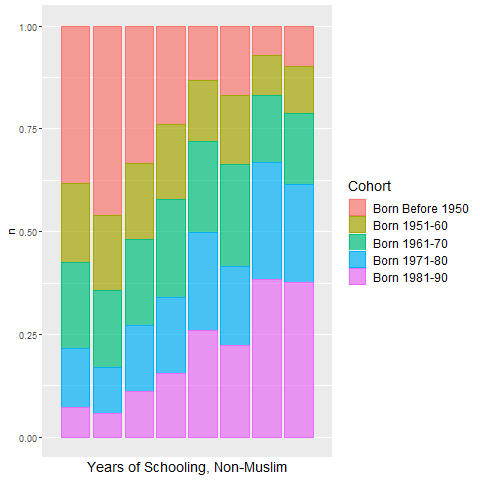
\includegraphics[width = \textwidth]{images/graph_edu_nonmus.png}
        \end{subfigure}
   \caption{Within group variation in levels of education, by cohort}
   \label{fig:within_group}
    \end{figure}

I describe the education gap between Hindus and Muslims in sample states in Table \ref{tab:across_group}. It is worth noting that mean levels of education are systematically lower among Muslims for all the cohorts. 


\begin{table}[H]
\resizebox{\textwidth}{!}{
\begin{tabular}{ccccccccccc}
\hline
Cohort Born & \multicolumn{2}{c}{Before 1950} & \multicolumn{2}{c}{1951-60} & \multicolumn{2}{c}{1961-70} & \multicolumn{2}{c}{1971-80} & \multicolumn{2}{c}{1981-90} \\ \hline
Whether Muslim   & No        & Yes      & No        & Yes      & No        & Yes      & No        & Yes      & No        & Yes      \\ \hline
Illiterate       & 30.02864  & 50.79830 & 18.09566  & 37.71874 & 14.84766  & 31.27104 & 10.33762  & 22.08000 & 5.42100   & 13.48787 \\
Primary School   & 58.19958  & 33.95423 & 74.38935  & 49.07731 & 78.89624  & 55.72391 & 84.90503  & 67.36000 & 91.14260  & 78.31379 \\
Middle School    & 45.62408  & 21.78020 & 62.85213  & 33.88482 & 67.63743  & 39.39394 & 75.87518  & 51.18000 & 83.33450  & 63.22384 \\
Secondary School & 35.22632  & 14.18308 & 48.84306  & 21.36494 & 51.97007  & 24.10564 & 58.68956  & 31.00000 & 63.68395  & 36.68666 \\
College          & 14.539067 & 4.350718 & 21.766857 & 6.745148 & 21.591673 & 7.070707 & 26.033095 & 8.640000 & 21.041856 & 7.106417 \\ \hline
\end{tabular}

}
\caption{Across group variation in level of schooling, by cohort}
\label{tab:across_group}
\end{table}


Furthermore, I slice the cohorts constructed by birth years into five-year intervals, to highlight the correlation between year of birth relative to the year 1990, and educational attainment. I expect educational choices for Muslim men born after 1971 to be affected differentially with distance from \textit{Yatra}.

\subsection{Segregation}
I measure segregation using the dissimilarity index \citep{massey.2018}. Residential segregation, for some city $c$, is measured as:

\begin{equation}\label{eq:dis_index}
d_c = \frac{1}{2} \sum_i \Bigl|\frac{m_{ic}}{M_c} - \frac{h_{ic}}{H_c}\Bigr|
\end{equation}

where, $m_{ic}$ is the Muslim population in city $c$ in neighbourhood $i$, $M_c$ is the total population of Muslims in city $c$, $h_{ic}$ is the non-Muslim population in city $c$ in neighbourhood $i$, and $H_c$ is the total population of non-Muslims in city $c$\footnote{See Appendix C for a detailed discussion.}.

\begin{figure}[h!]
    \centering
    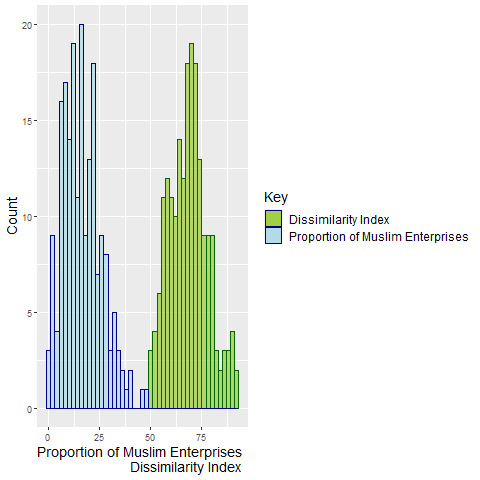
\includegraphics[scale=0.55]{images/graph_seg_dist.png}
    \caption{Distribution of dissimilarity indices, and Proportion of Muslim Enterprises across Indian cities}
    \label{fig:seg_dist}
\end{figure}

I construct this measure using religion indicators in the Sixth Economic Census conducted by the Ministry of Statistics and Program Implementation, Government of India \citep{ec.2013} for about 25 million residential and residential-cum-commercial enterprises all over India. This data is available at the level of enumeration block, where every EB has about 80 to 200 households. Figure \ref{fig:seg_dist} shows the distribution of the segregation measure and proportion of Muslim owned enterprises across Indian cities computed using this data.

\subsection{Town Level Attributes}
I link the Dissimilarity Indices  (from \eqref{eq:dis_index}), constructed using Economic Census, to Town Directories of the Population Census (1990, 2000 and 2010), compiled by the Ministry of Statistics and Program Implementation, Government of India \citep{td.2011}. The linking of the Economic Census and Population Census was done using Socio-Economic High Resolution Rural-Urban Geographic (SHRUG) Platform for India made freely available by \cite{almn2019}.

I use the Town Directories from the Population Census to get city level attributes like urban population, number of primary and secondary schools (both public and private), and number of colleges and universities, over time. 

Before moving on to the empirical strategy in Section \ref{empirical_strategy}, I summarize the variables of interest in Table \ref{tab:variables}.

\begin{table}[h!]
\centering
\begin{tabular}{ccccc}
\hline Variable Name & Notation & Across City & Across Households & Time/ Cohort  \\ 
    \midrule
    Distance from \textit{Yatra} Route &   $z_{c}$ & Yes & No & No \\
    Segregation Measure & $\theta_c$ & Yes & No & No \\
    Violence & $\rho_{c}$ & Yes & No & No \\
    Whether attained Education Level $e$ & $\sigma_{ihct}^e$ & Yes & Yes & Yes  \\
    Whether Muslim & $d_{ihc}$ & Yes & Yes & No \\
    City Controls & $X_{ct}$ & Yes & No & Yes \\
    Household Controls & $X_{hct}$ & Yes & Yes & Yes \\
    Household Consumption & $\kappa_{hct}$ & Yes & Yes & Yes \\
    \hline
\end{tabular}
\caption{Variation in variables on interest}
\label{tab:variables}
\end{table}

\section{Empirical Strategy}\label{empirical_strategy}
I measure the effect of communal violence on education attainment for Muslims in India. However, \cite{mitra.2014} demonstrate that rioting is correlated with relative incomes (measured by consumption expenditures) levels of Hindus and Muslims. This, in turn, is correlated with schooling choices, thus biasing the OLS estimates due to omitted variables. Therefore, I exploit quasi-random exposure of cities to communal violence. I obtain this variation in riots by tracing the path of the {Ram Rath Yatra} (1990), and check that distance from \textit{Yatra} is in fact uncorrelated with relative Muslim incomes over time\footnote{This helps to address valid issues raised by \cite{mitra.2014}. See Figure \ref{fig:mpce_yatra_muslim}.}. 

I propose my preferred instrument for communal violence: the distance of a town from the \emph{Yatra} route, as it actualized in reality. I restrict the sample to the states that were exposed to the \emph{Yatra} campaign. I have already demonstrated that a disproportionate share of riots in 1990-93 occurred on or very close to the \emph{Yatra} route in Figure \ref{fig:riots_yatra}.

First, I employ a random effects specification to establish the relationships between education outcomes and distance from \textit{Yatra}. Second, I demonstrate balance in control variables with respect to distance from \textit{Yatra} and specify a matching design with continuous treatments, to correct for selection on observables. Third, I lay out the design for robustness checks by administering placebo treatments. Fourth, I describe my strategy to test residential segregation as a channel through which communal violence impacts education outcomes. Finally, I write down the additional assumptions required to estimate the impact of segregation on education outcomes of Muslims, using distance from \textit{Yatra} as an instrument.

\subsection{Reduced Form Specification}\label{reduced_form}
I measure the relationship between Muslim education attainment and distance of a city from the \textit{Yatra} route. On account of the timing of the event (September-October, 1990), I expect different cohorts to respond to the event differently, by religion. In particular, cohorts born after 1985 are hypothesized to begin schooling after facing displacement on account of \textit{Yatra} riots. Cohorts born between 1981 and 1985 are assumed to already be in school by 1990. Cohorts born before 1971 would have completed schooling by this time. Then, the probability for Muslims of cohort $t$ to have attained education level $e$ is 

\begin{equation}
\begin{split}\label{eq:lpm_yatra}
       \sigma_{ihct}^e = \alpha + d_{ihc} + \gamma \log(z_c) + \sum_{t}\delta_{t} \mathbb{I(born = t)} + \\
       \sum_{t} \beta_{t} \log(z_c) \cdot \mathbb{I} (born = t) \cdot d_{ihc}+ \\
       \phi X_{hct} + \xi_{ct} + \varepsilon_{ihct} \\
\end{split}
\end{equation}

where, $\sigma_{ihct}^e \in \{0, 1\}$ indicates whether individual $i$ in household $h$, city $c$ and cohort $t$ attained education level $e \in$ \{Primary, Secondary or College\}, $d_{ihc}$ is dummy coded indicating whether household is Muslim, $t \in \{1951, 1961, 1971, 1981 \}$ depicts the cohort an individual belongs to and $\mathbb{I(\cdot)}$ is an indicator function, $z_c$ denotes distance of city $c$ from \textit{Yatra} route in kilometres, $X_{hc}$ and $\xi_{c}$ are household level controls and random effects for city $c$ respectively, $\varepsilon_{ihct}$ is the random error term. The pairs of cross-products from the triple difference term were dropped from \eqref{eq:lpm_yatra} for brevity, and cohorts of non-Muslim individuals born before 1951 are assumed to be the base category in this analysis. $\beta_t$'s are correctly estimated under the following assumptions: 

\begin{equation} \label{eq:a1} \tag{A1}
    \E[\xi_{ct} | \log(z_c)] = 0
\end{equation}

\begin{equation} \label{eq:a2} \tag{A2}
    \E[\xi_{ct} | \mathbb{I} (born = t)] = 0
\end{equation}

\begin{equation} \label{eq:a3} \tag{A3}
    \E[\xi_{ct} | d_{ihc}] = 0
\end{equation} 

These conditions imply that there are no time-varying unobservable characteristics of a city that vary with the distance from the campaign route in a discernible pattern \eqref{eq:a1}, or that impact various generation of cohorts \eqref{eq:a2} and Muslims \eqref{eq:a3} differently. In order to check the validity of these assumptions (and in the absence of unobservable city characteristics), I check how various time-varying observable characteristics of a city relate with $z_c$.

\eqref{eq:a2} is the most tenable assumption, as timing of birth is unrelated to city characteristics. However, Figure \ref{fig:pop_yatra} demonstrates that cities closer to the route are more populous (and larger), and in this way \eqref{eq:a1} may be violated. 

\begin{figure}[H]
    \centering
    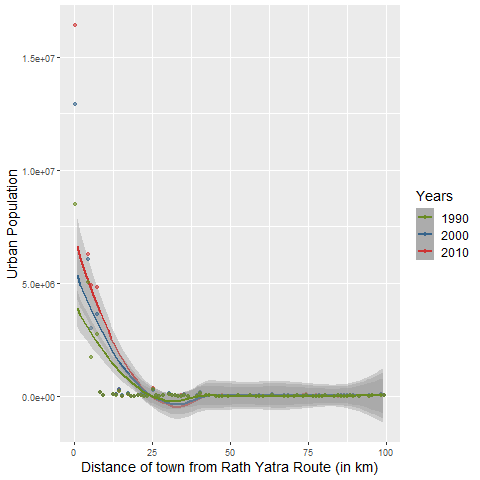
\includegraphics[scale = 0.7]{images/graph_pop_yatra.png}
    \caption{Total urban population as a function of Distance from \textit{Yatra}.}
    \label{fig:pop_yatra}
\end{figure}

I further divide the sample of cities within 250 kilometres of the \textit{Yatra} route into five subsamples, in intervals of 50 kilometres each. In Table \ref{tab:population_yatra}, I find that cities closest to the route (0 to 50 kilometres) are more populous in all three Census years under consideration. The remaining four groups, however, are indistinguishable in terms of urban population.  

 \begin{table}[H]
    \centering
    \resizebox{\textwidth}{!}{
    
\begin{tabular}{cccccc}
\cline{1-6}
 
  Distance from Yatra (in km) &
  \begin{tabular}[c]{@{}c@{}}0 to 50 \\ (N = 63)\end{tabular} &
  \begin{tabular}[c]{@{}c@{}}50 to 100 \\ (N = 52)\end{tabular} &
  \begin{tabular}[c]{@{}c@{}}100 to 150 \\ (N = 30)\end{tabular} &
  \begin{tabular}[c]{@{}c@{}}150 to 200 \\ (N = 21)\end{tabular} &
  \begin{tabular}[c]{@{}c@{}}200 to 250\\ (N = 16)\end{tabular} \\ \cline{2-6} 
   Urban Population & Mean (SD)           & Mean (SD)       & Mean (SD)       & Mean (SD)       & Mean (SD)       \\ \cline{1-6} 
 2010             & 860,772 (2,891,720) & 42,831 (21,389) & 51,719 (23,873) & 46,532 (22,279) & 61,608 (40,284) \\
 2000             & 711,609 (2,392,860) & 44,498 (18,465) & 52,610 (23,772) & 47,561 (21,078) & 69,836 (45,792) \\
 1990             & 528,602 (1,772,673) & 34,963 (12,855) & 41,373 (18,612) & 39,743 (22,183) & 51,743 (35,830) \\ \cline{1-6} 
\end{tabular}

    }
    \caption{Balance of Urban Population across groups (by distance from \textit{Yatra}).}
    \label{tab:population_yatra}
 \end{table}

Table \ref{tab:schools_yatra}, on the other hand, demonstrates that the most populous cities (which are closer to the \textit{Yatra} route) are not different from all other cities in terms of supply of school and college infrastructure, over the years. The difference in city size (by continuous treatment) can potentially bias my estimates, and I describe  strategies to address this problem in Section \ref{matching}. 

 \begin{table}[H]
    \centering
    \resizebox{\textwidth}{!}{
    
\begin{tabular}{cccccc}
\hline
Distance from Yatra (in km) &
  \begin{tabular}[c]{@{}c@{}}0 to 50 \\ (N = 63)\end{tabular} &
  \begin{tabular}[c]{@{}c@{}}50 to 100 \\ (N = 52)\end{tabular} &
  \begin{tabular}[c]{@{}c@{}}100 to 150 \\ (N = 30)\end{tabular} &
  \begin{tabular}[c]{@{}c@{}}150 to 200 \\ (N = 21)\end{tabular} &
  \begin{tabular}[c]{@{}c@{}}200-250 \\ (N = 16)\end{tabular} \\ \cline{2-6} 
Schools            & Mean (SD)     & Mean (SD)   & Mean (SD)   & Mean (SD)   & Mean (SD)   \\ \hline
\textbf{Primary}   &               &             &             &             &             \\
2010               & 4.64 (2.27)	& 5.81 (2.38)	& 5.43 (2.02) &	5.73 (2.48) &	6.01 (1.95) \\
2000               & 4.14 (2.33) &	3.94 (1.22) &	3.80 (1.31) &	4.18 (1.66) &	5.09 (5.05)  \\
1990               & 3.47 (1.28) &	3.70 (0.98) &	3.38 (1.07) &	4.16 (1.83)	& 3.77 (1.80)    \\ \hline
\textbf{Secondary} &               &             &             &             &             \\
2010               & 1.62 (0.88) &	2.19 (1.18) &	2.05 (1.00) &	1.84 (0.73) &	1.96 (0.71)  \\
2000               & 1.35 (0.71) &	1.34 (0.60) &	1.27 (0.81) &	1.58 (0.68) &	1.30 (0.61) \\
1990               & 1.15 (0.51) &	1.17 (0.45) &	1.07 (0.42) &	1.20 (0.37) &	0.95 (0.46)  \\ \hline
\textbf{College}   &               &             &             &             &             \\
2010               & 0.79 (0.46) &	1.06 (0.62) &	1.04 (0.71) &	0.67 (0.41) &	0.97 (0.71)   \\
2000               & 0.41 (0.40) &	0.45 (0.20)	& 0.41 (0.29)	& 0.37 (0.18)	& 0.39 (0.15) \\
1990               & 0.65 (0.41) &	0.82 (0.48) &	0.83 (1.04) & 0.80 (0.42) &	0.67 (0.42) \\
\hline
\end{tabular}

    }
    \caption{Balance of school and college infrastructure, per 10,000 urban residents (by distance from \textit{Yatra}).}
    \label{tab:schools_yatra}
 \end{table}
 
Next, I discuss the credibility of assumption \ref{eq:a3}. That is, I check if there are time-varying city characteristics that vary with proportion of urban Muslim population. In Figure \ref{fig:permuslim_yatra}, I plot the percentage share of Muslims sampled in the NSS surveys over the years, as well as percentage of Muslim enterprises from the Economic Census in 2013.
 
 \begin{figure}[H]
     \centering
     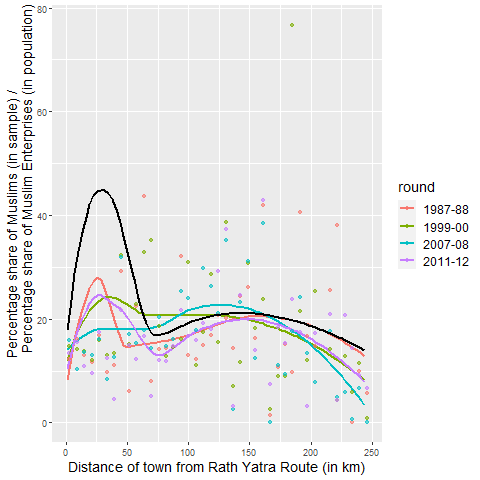
\includegraphics[scale = 0.6]{images/graph_permuslim.png}
     \caption{Proportion of Muslim households in NSSO samples over various round, and Muslim enterprises in Economic Census (black solid line) in 2013, by distance from \textit{Yatra} route.}
     \label{fig:permuslim_yatra}
 \end{figure}
 
 From Figure \ref{fig:permuslim_yatra}, I cannot conclude that Muslim population is distributed differently by distance, pre- and post-1990. It is, however, clear that the odds of finding Muslim-owned enterprises are higher within the first 50 kilometres of the \textit{Yatra} route in the year 2013. Another important household characteristic is income, which I proxy with Monthly Per Capita Expenditures (hencefoth, MPCE). Figure \ref{fig:mpce_yatra_muslim} shows that there is no relationship between the instrument and MPCE (normalized to 1983 Rupees), over the years. 
 
 \begin{figure}[H]
     \centering
     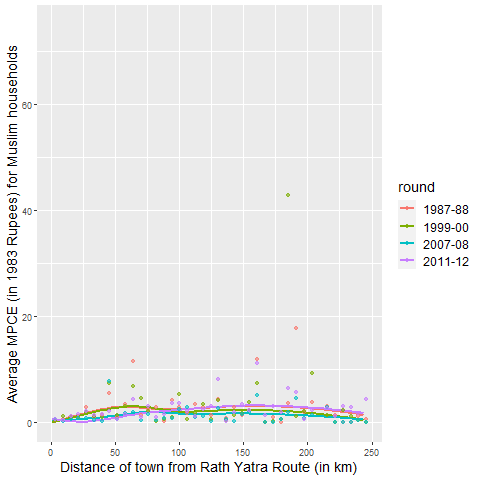
\includegraphics[scale = 0.6]{images/graph_mpce_yatra_muslim.png}
     \caption{Muslim Monthly Per Capita Consumption (in 1983 Rupees) relative to non-Muslim MPCE, as a function of distance from \textit{Yatra} route.}
     \label{fig:mpce_yatra_muslim}
 \end{figure}
 
 This assuages the threat to identification raised by \cite{mitra.2014}, who found that higher Muslim MPCEs relative to Hindu MPCEs, were correlated with the higher probability of communal violence. This is because, in my sample, the probability of a riot is higher closer to the campaign route, but average Muslim MPCEs (relative to non-Muslim MPCEs) seem to be uniformly distributed in the sample, both pre- and post-\textit{Yatra}.

\subsection{Matching Design}\label{matching}
Using various observable characteristics of  the sample cities, I demonstrated in Section \ref{reduced_form} that cities closer to the \textit{Yatra} route are more populous (and bigger), than cities away from it. I also showed that it was more likely to find a Muslim-owned enterprise in the first 50 kilometres of the \textit{Yatra} route, in the post-treatment period. Therefore, I estimate the model in \eqref{eq:lpm_yatra} by matching propensity scores calibrated for continuous treatment, following \cite{hirano2004propensity}.

To remain consistent with standard notation in the literature, I denote potential outcomes as $Y_{ihtc}(z_c)$ (education outcomes, previously denoted as $\sigma_{ihtc}^e$), for $z \in Z$, where $Z$ is continuous treatment (distance from \textit{Yatra} route) in interval $[z_0, z_1]$. Dropping subscripts, the main assumption is described as

\begin{equation}\label{eq:a4} \tag{A4}
    Y(z) \perp Z | X \textrm{ for all } z \in Z
\end{equation}
where, $X$ denotes various city level controls. Then under \eqref{eq:a4}, I define the generalized propensity score (GPS), $R = r(Z, X)$ as the conditional density of the treatment conditional on covariates, i.e.

\begin{equation}
    r(z, x) = f_{Z | X} (z | x)
\end{equation}

Then, $X \perp 1\{Z = z\} | r(z, X)$, which implies that assignment to treatment is not confounded, given the GPS. That is,
$$f_Z(z|r(z, X), Y(z)) = f_Z(z | r(z, X))$$

Following \cite{robins2000marginal}, I calculate stabilized inverse probability weights (henceforth, IPW) as:
\begin{equation}
    \iota^s = \frac{f_Z^{(z)}}{f_{Z | X}^{(z | x)}}
\end{equation}

Assuming $Z_c | X_c \sim N(\beta_0 + \beta'_1 X_c, \sigma^2)$, with $X_c$ being city level attributes like urban population in 1990,  I estimate stabilized IPWs \footnote{I fit the distribution of continuous treatment with a function that is piece-wise linear in urban population of 1990, by estimating a spline regression.}. Furthermore, I plot the density of $\iota^s$ in Figure \ref{fig:ipw_s}, and find that it is centred around 1.  

\begin{figure}[H]
    \centering
    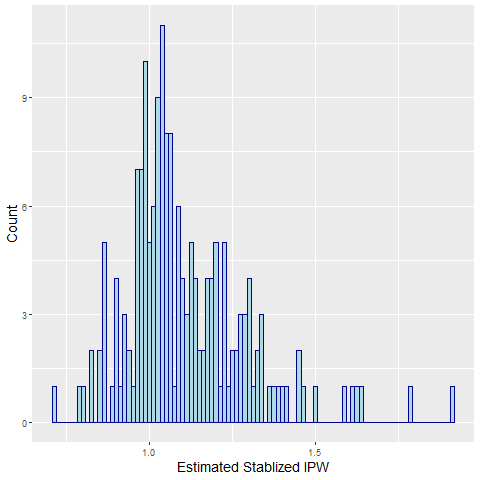
\includegraphics[scale = 0.6]{images/graph_ipw_dist.png}
    \caption{Sample distribution of estimated Stabilized Inverse Probability Weights (IPW).}
    \label{fig:ipw_s}
\end{figure}

Further, I check if stabilized IPWs are systematically related with the treatment. In Figure \ref{fig:ipw_yatra}, I do not find that the weights co-vary with the continuous treatment in an identifiable way. This grants greater credibility to the research design.

\begin{figure}[H]
    \centering
    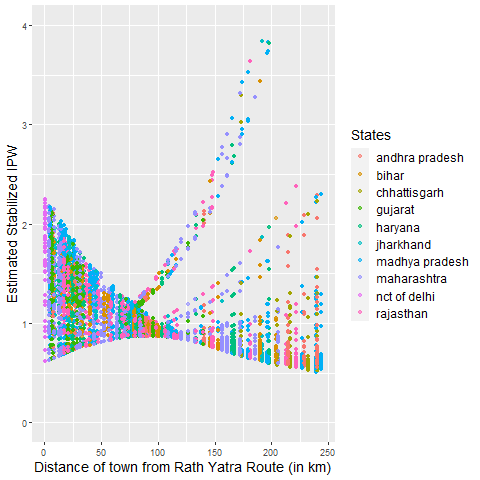
\includegraphics[scale = 0.6]{images/graph_ipw_yatra.png}
    \caption{Correlation between estimated Stabilized Inverse Probability Weights (IPWs) and distance from \textit{Yatra} route}
    \label{fig:ipw_yatra}
\end{figure}

\subsection{Placebo \textit{Yatra}}\label{strategy_placebo}
On October 23, 1990, the state government of Bihar issued orders to arrest prominent BJP leader, LK Advani, who was spearheading the \emph{Ram Janmabhoomi} campaign \citep{lalu}. This brought the \emph{Ram Rath Yatra} to an unexpected halt, a week before it was supposed to reach it's final destination in Ayodhya, UP. I exploit exogeneity in the timing (and therefore, the location) of this arrest, to construct a placebo treatment. This is done by charting out the \textit{planned} route which the campaign was unable to tread due to this arrest. I find no correlation between the placebo route and the number of riots occurring in a city until the ultimate demolition of \textit{Babri Masjid} in December, 1992. 

\begin{figure}[H]
    \centering
    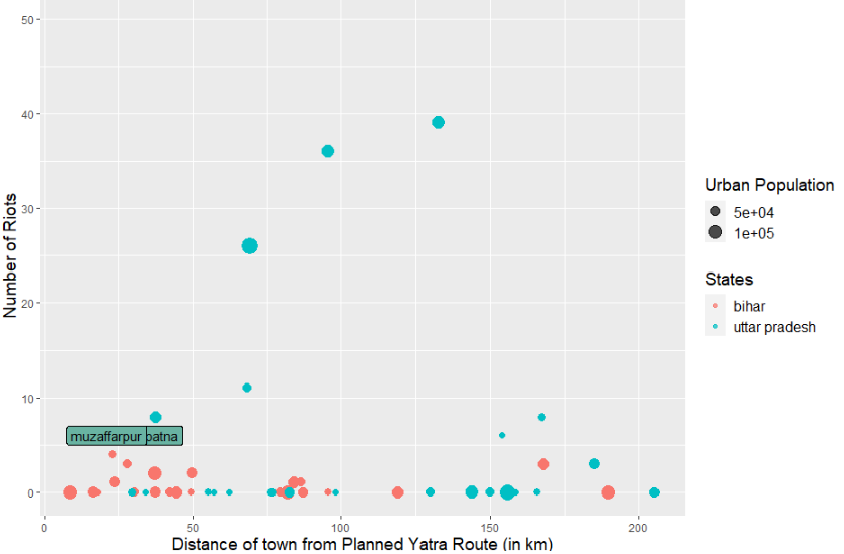
\includegraphics[scale = 0.6]{images/graph_riots_yatra_p.png}
    \caption{Number of riots (1990-93) by distance from \textit{placebo Yatra} route.}
    \label{fig:riots_yatra_p}
\end{figure}

Figure \ref{fig:riots_yatra_p} presents a contrasting picture with respect to Figure \ref{fig:riots_yatra}, where I saw a strong and negative relationship between rioting and the continuous treatment. It is worth mentioning that rioting occurred in the labelled districts of Patna and Muzaffarpur, that are close to the placebo route. However, note that both these districts are right next to Samastipur district, where LK Advani was in fact arrested. It is therefore, more likely, that rioting here was on account of the treatment, and not the placebo.

Then, I estimate the reduced-form equation \eqref{eq:lpm_yatra} again, this time with respect to distance from the placebo \textit{Yatra}

%\begin{equation}\label{eq:fs_p}
%    \theta_c = \alpha + \log(z_c^P) + \psi X_{c} + \mu_c
%\end{equation}

\begin{equation}
\begin{split}\label{eq:lpm_yatra_p}
       \sigma_{ihct}^e = \alpha + d_{ihc} + \gamma \log(z_c^P) + \sum_{t}\delta_{t} \mathbb{I(born = t)} + \\
       \sum_{t} \beta_{t} \log(z_c^P) \cdot \mathbb{I} (born = t) \cdot d_{ihc}+ \\
       \phi X_{hct} + \xi_{ct} + \varepsilon_{ihct} \\
\end{split}
\end{equation}

where, $z_c^P$ denotes the placebo \textit{Yatra} route, and the remaining notation from above remains the same.

\subsection{Channels: Neighbourhood Effects}\label{channels}

In light of the reduced form results obtained from the specifications above, I explore if segregation of communities along religious lines drives the effects of violence on Muslim education outcomes. I estimate the static relationship between segregation ($\theta_c$) and distance from the route ($z_c$), while controlling for city level observables ($X_c$) as:

\begin{equation}\label{eq:fs}
    \theta_c = \alpha + \tau \log(z_c) + \psi X_{c} + \mu_c
\end{equation}

I also estimate the relationship between segregation and the placebo, that is the distance from the planned \textit{Yatra} route, and this lends greater credibility to the stipulated channel. Additionally, I verify that there is no treatment effect on untreated groups like Scheduled Castes, as I test the hypothesis that distance of a city from \textit{Yatra} route is uncorrelated with dissimilarity index constructed according to caste and not religion. 

I hypothesize that segregation of Muslim and Hindu neighbourhoods in Indian cities drives better early education outcomes for Muslims in locations that were more susceptible to communal conflict. The ideal experiment to uncover causal effects of neighbourhood characteristics on individual education outcomes, would assign the opportunity to live in segregated or integrated neighbourhoods randomly. However, in addition to manipulating the composition of neighbourhoods, communal violence along the campaign trail may change the political environment in a way that changes the likelihood of going to school, for different groups differently. 

Following \cite{abdulkadirouglu2014elite}, I postulate a vector $m_{ic}$ assumed to contain education inputs like composition of neighbourhood, parental income, measures of school quality, and political environment or discriminatory attitudes towards Muslims. Then, the education production function, dropping cohort subscripts, is given by 
$$\sigma_{ic}^e = \pi ' m_{ic} + \eta_{ic}$$
where, $\eta_{ic}$ is the randomness in potential outcomes revealed under alternative assignments of the input bundle $m_{ic}$ for individual $i$, residing in city $c$. Furthermore, I can partition $m_{ic}$ into observed segregation levels for a Muslim individual $i$ in city $c $, $\theta_{ic}$, as well as unobserved inputs $w_{ic}$. Then, the structural education production function can be written as:

\begin{equation}\label{eq:unobservables}
    \sigma_{ic}^e = \delta' \theta_{ic} + \lambda' w_{ic} + \eta_{ic}
\end{equation}

where, $\theta_{ic}$ is dissimilarity index ($\theta_c$) interacted with a dummy variable that is equal to 1 for Muslims ($d_{ic}$). Then, the instrumental variable, $z_{ic}$, is given by distance of a city from \textit{Yatra} route ($z_c$) interacted with the Muslim dummy. Here, I assume that the instrument is independent of potential outcomes, i.e. independent of $\eta_{ic}$. However, the instrument does not meet the exclusion restriction as not only does \textit{Yatra} change the composition of neighbourhoods, it also changes unobserved inputs in \eqref{eq:unobservables}. That is,
$$\theta_{ic} =  \omega_1' z_{ic} + \nu_{1c}$$
$$w_{ic} = \omega_2' z_{ic} + \nu_{2c}$$

With this structure, the 2SLS estimate using $z_{ic}$ as an instrument for $\theta_{ic}$, omitting $w_{ic}$ identifies $\delta + u' \lambda$, where $u$ is the population 2SLS coefficient vector from a regression of $w_{ic}$ on $\theta_{ic}$, using $z_{ic}$ as instrument\footnote{see Proposition 1 in \cite{abdulkadirouglu2014elite}.}. Then, suppose if $u$ and $\lambda$ are  positive, 2SLS estimates of neighbourhood effects, omitting $w_{ic}$, tend to be too big. 

Building on the existing literature, I will provide evidence that $\lambda$ is in fact negative, while maintaining the assumption that $u > 0$. That is to say, while the unobservables co-vary with the segregation measure, $w_{ic}$ impacts education outcomes negatively. Therefore, under weaker assumptions on the bias induced by unobserved inputs in the education production function, I will show in Section \ref{results}, that the direction of neighbourhood effects on Muslim education attainment is positive.  

\subsection{IV Specification}
I am interested in uncovering the relationship between education levels of Muslims and residential segregation associated with communal violence on account of the 1990 campaign. The linear probability model for completing education level $e$, as a function of segregation, is given by

\begin{equation}
\begin{split}\label{eq:lpm}
       \sigma_{ihct}^e = \alpha + d_{ihc} + \gamma \theta_c + \sum_{t}\delta_{t} \mathbb{I(born = t)} + \\
       \sum_{t} \beta_{t} \theta_c \cdot \mathbb{I} (born = t) \cdot d_{ihc}+ \\
       \phi X_{hct} + \psi X_{ct} + \varepsilon_{ihct} \\
\end{split}
\end{equation}

As before, $\sigma_{ihct}^e \in \{0, 1\}$ indicates whether individual $i$ in household $h$, city $c$ and cohort $t$ attained education level $e \in$ \{Primary, Secondary or College\}, $d_{ihc}$ is dummy coded indicating whether household is Muslim, $t \in \{1951, 1961, 1971, 1981 \}$ depicts the cohort an individual belongs to and $\mathbb{I(\cdot)}$ is an indicator function, $\theta_c$ is the dissimilarity index (expressed in percentage terms), $X_{hc}$ and $X_{c}$ are household and city level controls respectively, $\varepsilon_{ihct}$ is the random error term. Cohorts of non-Muslim individuals born before 1951 are assumed to be the base category for this analysis.

The estimates from linear probability model ($\hat{\beta}_t$'s from \eqref{eq:lpm} are likely to be biased as residential choices are correlated with schooling choices that parents make for their children. Therefore, I exploit variation in residential choices caused by displacement due to communal violence on account of \textit{Yatra}. 

 In order to understand the impact of residential segregation on education outcomes of Muslims, I re-state the first stage of my Instrumental Variable Regression as 

\begin{equation}\label{eq:fs_iv}\tag{$\star$}
    \theta_c = \alpha + \tau \log(z_c) + \psi X_{c} + \mu_c
\end{equation}

The exclusion restriction would require that
\begin{equation}\label{eq:a5}\tag{A5}
    \E[\mu_c | z_c, X_c] = 0
\end{equation}

That is to say, I assume that the actual \emph{Yatra} route was exogenously determined. Then, the structural relationship of interest is

\begin{equation}\label{eq:lpm_yatra_iv} \tag{$\star \star$}
\begin{split}
       \sigma_{ihct}^e = \alpha + d_{ihc} + \gamma \hat{\theta}_c + \sum_{t}\delta_{t} \mathbb{I(born = t)} + \\
       \sum_{t} \beta_{t} \hat{\theta}_c \cdot \mathbb{I} (born = t) \cdot d_{ihc}+ \\
       \phi X_{hct} + \xi_{ct} + \varepsilon_{ihct} \\
\end{split}
\end{equation}

where $\hat{\theta}_c$ is estimated in \eqref{eq:fs_iv}. For this specification, I assume that the only channel through which distance from \emph{Yatra} influences education outcomes for Muslims, is through residential segregation. I will then relax this assumption in line with section \ref{channels}, and show that the neighbourhood effects are positive. Next, I turn to the obtained results.

\section{Results}\label{results}
In this Section, I implement the empirical strategy delineated in Section \ref{empirical_strategy}.

\subsection{Reduced Form Specification}\label{reduced_form_results}
In order to correctly estimate \eqref{eq:lpm_yatra}, I want to ensure that the education levels of cohorts (both Muslims and Non-Muslims) attending school prior to 1990, are not affected differently. That is, I expect education levels of Muslims born after 1971 (aged between 0 to 19 in 1990) to be differentially impacted by distance of their city to \textit{Yatra} route. In Figure \ref{fig:li_pri_mus}, I find parallel trends in the probability that Muslims and Non-Muslims attend Primary School with respect to the treatment, for cohorts who had already finished schooling by 1990 (Those born before 1971).

\begin{figure}[H]
    \centering
    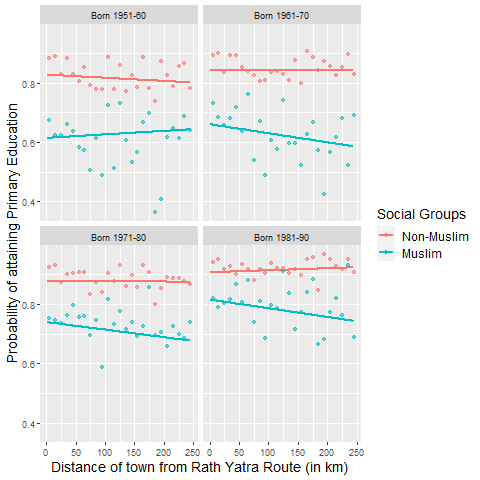
\includegraphics[scale = 0.7]{images/graph_li_pri_mus.png}
    \caption{Probability of attaining primary education by religion, cohort, and distance from \textit{Yatra}}
    \label{fig:li_pri_mus}
\end{figure}

I check if the parallel trends assumption is satisfied for other outcome variables, namely probability of attending secondary school and college in Appendix Figures \ref{fig:li_sec_mus} and \ref{fig:li_col_mus}. I estimate \ref{eq:lpm_yatra}, and present estimates corresponding to completion of primary school in Figure \ref{fig:coeff_pri}.

\begin{figure}[H]
    \centering
    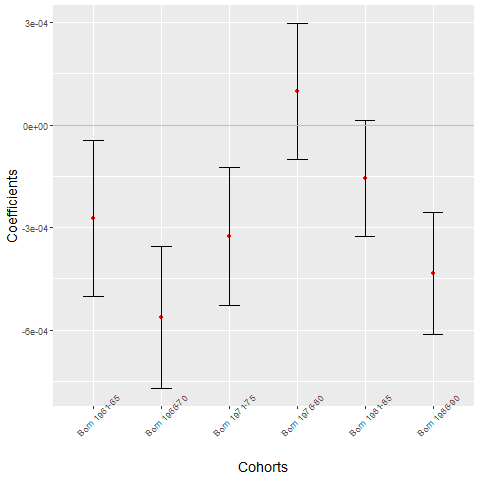
\includegraphics[scale = 0.6]{images/graph_coeff_pri.png}
    \caption{$\hat{\beta}$'s estimated from \eqref{eq:lpm_yatra}, for completion of primary school.}
    \label{fig:coeff_pri}
\end{figure}

For cohorts born after 1981, I find a significantly negative relationship between distance from \textit{Yatra} and probability of attaining primary education, for Muslims. The corresponding graphs for illiteracy, and attainment of secondary and college education are in Appendix A (Figures \ref{fig:coeff_ill}, \ref{fig:coeff_sec}, and \ref{fig:coeff_col}). 

I find that Muslims born in cities away from the campaign route, after the year 1980, face a disadvantage in terms of early education. However, I find that Muslims born between 1981-85 face an advantage in attainment of secondary education (conditional on having completed middle school) farther away from the campaign route, while Muslims born between 1986-90 face a similar advantage for college education, conditional on having completed secondary school.

\subsection{Matching Design}\label{matching_results}
I implement the research design laid out in Section \ref{matching} by reweighting the reduced form equation in \eqref{eq:lpm_yatra} using the Stabilized Inverse Probability Weights (IPWs) in \eqref{fig:ipw_s} from the Generalized Propensity Scores (GPS). The sample distribution of estimated IPWs is given by Figure \ref{fig:ipw_s}, and the absence of correlation between the weights and the treatment is demonstrated by Figure \ref{fig:ipw_yatra}.

In Table \ref{tab:education_score_re}, I summarize the relationship between education levels of Muslims born after 1980 with respect to the continuous treatment, weighted by IPWs. I find that all the estimates are still significant (except College attendance for Muslims of Cohort born 1986-90), and have the same signs as corresponding estimates in Table \ref{tab:education_re}. However, the unweighted estimates seem to have been systematically biased upwards as the absolute value of weighted estimates is now smaller in magnitude. I provide estimates weighted by IPW, for all other cohorts in Table \ref{tab:education_score_re_old}. 

\begin{table}[H]
    \centering
    {
\def\sym#1{\ifmmode^{#1}\else\(^{#1}\)\fi}
\begin{tabular}{l*{2}{c}}
\hline\hline
            &\multicolumn{1}{c}{(1)}&\multicolumn{1}{c}{(2)}\\
            &\multicolumn{1}{c}{Born 1981-85}&\multicolumn{1}{c}{Born 1986-90}\\
[1em]
\hline
\textbf{Illiteracy Level} & & \\
[1em]
\textit{Yatra} distance $\times$ Muslim &    0.000163\sym{*} &    0.000177\sym{*}  \\
            &  (0.0000819)         & (0.0000837)         \\
[1em]
\hline
\textbf{Primary School} & & \\
[1em]
&   -0.000183\sym{*} &  -0.000203\sym{*} \\
& (0.0000845)         & (0.0000864)         \\
[1em]
\hline
\textbf{Secondary School} & & \\
[1em]
&    0.000556\sym{**} &    0.000231         \\
&  (0.000192)         &  (0.000185)         \\
[1em]
\hline
\textbf{College} & & \\
[1em]
&    0.000187 &    0.000427\\
&  (0.000270) &  (0.000253)\\
[1em]
\hline\hline
\multicolumn{3}{l}{\footnotesize Standard errors in parentheses}\\
\multicolumn{3}{l}{\footnotesize \sym{*} \(p<0.05\), \sym{**} \(p<0.01\), \sym{***} \(p<0.001\)}\\
\end{tabular}
}
    \caption{Relationship between distance from \textit{Yatra} route (in km) and education attainment levels for Muslims born after 1980, weighted by stabilized IPW.}
    \label{tab:education_score_re}
\end{table}

\subsection{Placebo \textit{Yatra}}
I use the arrest of BJP leader, LK Advani, and the subsequent suspension of the campaign to identify parts of the planned route that did not actually see the \textit{Yatra}. As elaborated in Section \ref{strategy_placebo}, this enables me to construct a placebo test, wherein I check if the same reduced form relationships hold in \eqref{eq:lpm_yatra_p} for the \textit{planned}, as opposed to the actual \textit{Yatra} route. 

I check if the relationship between the placebo route, and education attainment level of Muslims from various cohorts follows patterns similar to cases when the treatment was actually administered (See Figures \ref{fig:li_pri_mus} and \ref{fig:coeff_pri}). I find that the relationship between primary education attainment and the placebo route is parallel for Muslims and non-Muslims of cohorts born after 1980 (Figure \ref{fig:li_pri_mus_p}), and does not mirror the effects of the treatment. Corresponding graphs for secondary and tertiary education attainment are given by Figures \ref{fig:li_sec_mus_p} and \ref{fig:li_col_mus_p}.

\begin{figure}[H]
    \centering
    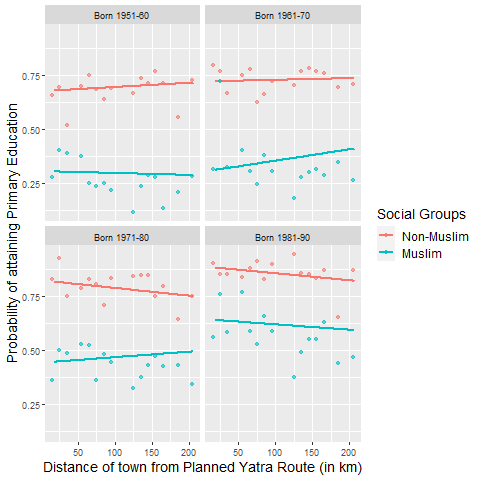
\includegraphics[scale = 0.7]{images/graph_li_pri_mus_p.png}
    \caption{Probability of attaining primary education by religion, cohort, and distance from \textit{placebo Yatra}.}
    \label{fig:li_pri_mus_p}
\end{figure}

Finally, I slice the cohorts by 5-year birth intervals and plot the coefficients estimated from \eqref{eq:lpm_yatra_p} in Figure \ref{fig:coeff_pri_p}. None of the coefficients are significantly different from zero, and I plot the corresponding coefficients for illiteracy, secondary and college education in Figures \ref{fig:coeff_ill_p}, \ref{fig:coeff_sec_p}, and \ref{fig:coeff_col_p}, respectively.

\begin{figure}[H]
    \centering
    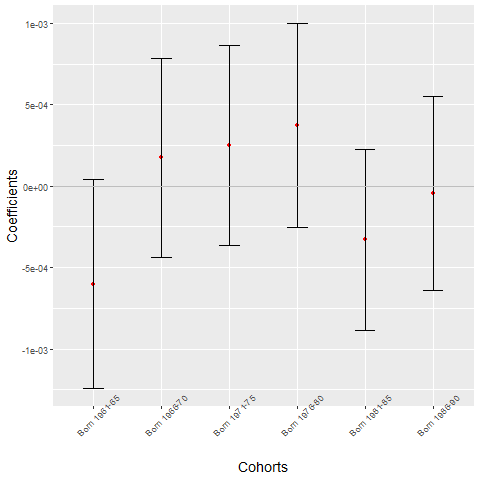
\includegraphics[scale = 0.6]{images/graph_coeff_pri_p.png}
    \caption{$\hat{\beta}$'s estimated from \eqref{eq:lpm_yatra_p} with respect to \textit{placebo Yatra}, for completion of primary school.}
    \label{fig:coeff_pri_p}
\end{figure}

Therefore, I have shown that the placebo route has no effects on the outcome variable of interest. This strengthens the reduced form results that were presented in Sections \ref{reduced_form_results} and \ref{matching_results}.

\subsection{Channels}
I argue that segregation along religious lines is a channel driving the very surprising and positive effects of communal violence on early education outcomes for Muslims. First, I estimate \eqref{eq:fs} and analyze the relationship between the continuous treatment and my measure of segregation in Figure \ref{fig:disindex_yatra}. In Table \ref{tab:disindex_yatra}, I provide estimates from OLS regressions without city level controls (in column 1), and while  controlling for population and proportion of Muslim owned enterprises (columns 2 and 3 respectively). In column 4, I regress the dissimilarity index on log of \textit{Yatra} distance. In all four cases, I find that the coefficient on the treatment is statistically significant, and negative. 

\begin{figure}[H]
    \centering
    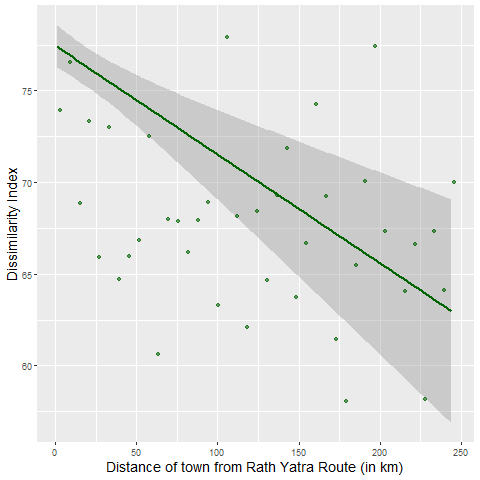
\includegraphics[scale = 0.6]{images/graph_disindex.png}
    \caption{Segregation measure (Dissimilarity Index $\times 100$) by Distance from \textit{Yatra} route.}
    \label{fig:disindex_yatra}
\end{figure}

Therefore, I can reject the null hypothesis of zero linear relationship between segregation and distance of city from campaign route, as I find a significant and negative relationship between the two. Additionally, the specification in column 4 of Table \ref{tab:disindex_yatra} seems to be the best fit. 

\begin{table}[H]
 \centering
\resizebox{\textwidth}{!}{
   {
\def\sym#1{\ifmmode^{#1}\else\(^{#1}\)\fi}
\begin{tabular}{l*{3}{c}}
\hline\hline
            &\multicolumn{1}{c}{(1)}&\multicolumn{1}{c}{(2)}&\multicolumn{1}{c}{(3)}\\
[1em]
\hline
Distance from \textit{Yatra} (in km) &      -.023836\sym{*}  &          -0.0206\sym{*}  &                     \\
            &    (0.0105)          &   (0.0104)         &                     \\
[1em]
Log of Distance from \textit{Yatra}   &                      &                     &      -1.832\sym{*} \\
            &                     &                     &     (0.706)         \\
[1em]
\hline
Population Controls      &       NO &  YES & NO \\
[1em]
Muslim Enterprise Controls      &       NO &  YES & NO \\
 
\hline
\(N\)       &         177         &         177         &         177         \\
F           &       4.181          &       5.112         &       6.729         \\
\hline\hline
\multicolumn{4}{l}{\footnotesize Standard errors in parentheses}\\
\multicolumn{4}{l}{\footnotesize \sym{*} \(p<0.05\), \sym{**} \(p<0.01\), \sym{***} \(p<0.001\)}\\
\end{tabular}
}

   }
    \caption{OLS estimates from regression of Segregation Measure (Dissimilarity Index $\times 100$) on Distance from \textit{Yatra}, with city level controls}
    \label{tab:disindex_yatra}
\end{table}

Second, I demonstrate that the same relationship does not hold with respect to the placebo. Figure \ref{fig:disindex_p} shows that in Uttar Pradesh, the segregation measure is in fact positively correlated with distance from the placebo route. This is not surprising, as Figure \ref{fig:riots_yatra_p} shows that in UP, displacement on account of riots was not more likely to occur closer to the \textit{planned} route.

\begin{figure}[H]
    \centering
    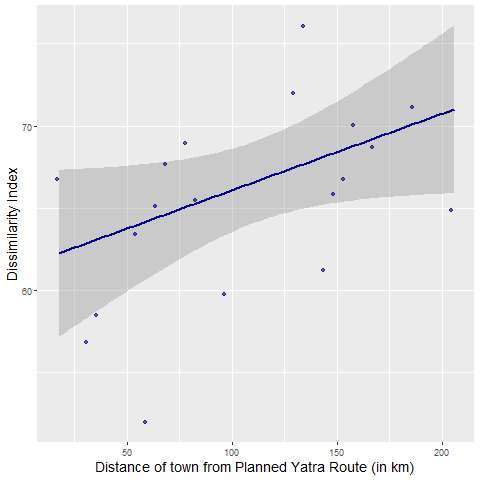
\includegraphics[scale = 0.6]{images/graph_disindex_p.png}
    \caption{Segregation measure (Dissimilarity Index $\times$ 100) by Distance from \textit{placebo Yatra} route.}
    \label{fig:disindex_p}
\end{figure}

Finally, I verify that there is no treatment effect on untreated groups. I have used quasi-random variation in communal violence to measure community (or religion) based segregation, as this is a displacement shock that affects Muslims only. In order to verify this, I check if the events of 1990 have any import on residential segregation of Scheduled Castes, who have also been documented to live in segregated enclaves \citep{bharathi2018isolated} but are not expected to get displaced due to communal conflicts. I construct caste based dissimilarity indices, using residential and residential-cum-commercial enterprises owned by Scheduled Castes in the Sixth Economic Census (2013).

In Figure \ref{fig:sc_disindex}, I do not find a statistically significant and negative relationship between caste-based segregation and distance from \textit{Yatra}. This lends credence to the story that displacement shocks due to \textit{Yatra} affected Muslims differently. 

\begin{figure}[H]
    \centering
    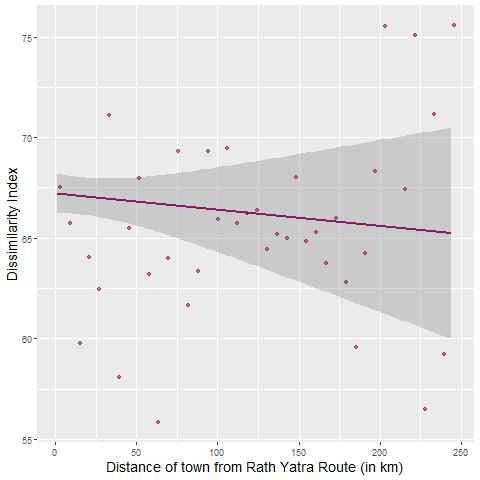
\includegraphics[scale = 0.6]{images/graph_sc_disindex.png}
    \caption{Relationship between caste-based segregation measure (dissimilarity index for scheduled caster $\times$ 100) and distance from \textit{Yatra} route in kilometres.}
    \label{fig:sc_disindex}
\end{figure}

Furthermore, I perform robustness checks to show that there is no evidence that education outcomes of the untreated group were differentially affected by quasi-random exposure to violence. This is evidenced by the absence of reduced form relationship between distance from \textit{Yatra} and differences in primary education attainment between Muslims and non-Muslims in Figure \ref{fig:li_pri_sc}. 

\subsection{IV Estimates}
Taking stock of the reduced form estimates in this Section, I now estimate the structural relationship described in \eqref{eq:lpm_yatra_iv}, where I instrument the segregation measure with distance from \textit{Yatra} route (according to the first-stage relationship in \eqref{eq:fs_iv}).

Table \ref{tab:disindex_yatra} makes a convincing case for a strong first-stage relationship. In \eqref{eq:a5}, I assume that $\E [ \mu_c | z_c, X_c ]$. That is to say, conditional on various town characteristics, the only channel through which the treatment impacts education levels is that of segregation. I will later relax this exclusion restriction and show that results remain consistent. 

Figure \ref{fig:coeff_pri_iv} shows that increased segregation leads to increased probability that Muslims born after 1981 attain primary education. Figures \ref{fig:coeff_ill_iv}, \ref{fig:coeff_sec_iv}, and \ref{fig:coeff_col_iv} provide the relationship between dissimilarity index and illiteracy levels, completion of secondary and tertiary education for Muslims of various cohorts, respectively. 

\begin{figure}[H]
    \centering
    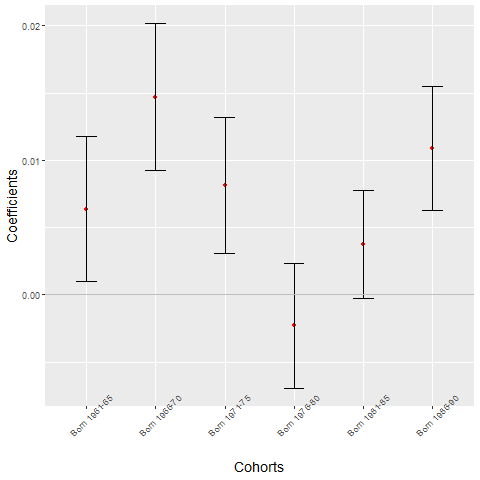
\includegraphics[scale = 0.6]{images/graph_coeff_pri_iv.png}
    \caption{IV estimates of $\hat{\beta}$'s from \eqref{eq:lpm_yatra_iv}, for completion of primary school.}
    \label{fig:coeff_pri_iv}
\end{figure}

I find that these results are consistent with the reduced form estimates above, wherein communal violence closer to the \textit{Yatra} route may have displaced Muslims into ethnic enclaves, where Muslim children going to school after 1990 also achieved higher levels of primary education. This may be due to presence of role models from the same community in these ethnic enclaves. These role models in the neighbourhood may have enabled Muslims to achieve higher levels of early education. However, as described in Section \ref{channels}, the exclusion restriction may be violated in the presence of unobservable inputs in the education production function if such inputs are also determined by distance of the city from \textit{Yatra}. 

I build upon previous work in the literature to argue that unobservable inputs (like political environment) in the education production function (those that are correlated with the instrument) have an effect that is diametrically opposed to that of segregation. First, notice that \cite{blakeslee.2018} finds significant electoral gains for the BJP in constituencies through which the \textit{Yatra} passed. He finds a 6 percentage point increase in the party's vote share, and an 11 percentage point increase in their probability of victory in elections. Similarly, \cite{iyer2015religious} demonstrates a 5 percentage points increase in the vote share of the BJP associated with exogenous variation in Hindu-Muslim riots. So, it is clear that the instrument is associated with electoral gains for the Hindu nationalist BJP. 

While communal riots cause much damage to life and property of Muslims, my second observation deals with worsening (or lack of improvement) in employment, consumption and education outcomes of Muslims in BJP ruled constituencies \citep{mitul2020bjp}. \cite{farooqui2020political} contends that the rise of BJP in the Indian political arena has grossly aggravated the under-representation of Muslims in politics, and this may be associated with worsening provision of public goods for this community. That is to say, unobservable political climate closer to the \textit{Yatra} route must necessarily correlate with Muslim education outcomes negatively, as the communal riots in these areas may have caused greater harm to Muslim life and property (direct channel) or led to electoral gains for BJP (indirect channel), which could not have improved Muslim education outcomes.  

Additionally, I have provided evidence in Figure \ref{fig:mpce_yatra_muslim} that household consumption for Muslims is not significantly different by treatment, pre or post- \textit{Yatra}. Then it must be the case that $\lambda \leq 0$. However, notice in Figure \ref{fig:coeff_pri_iv} IV estimates for attainment of primary education, for cohorts born between 1981-90, imply that

\begin{equation}\label{eq:causal}
\delta + u' \cdot \lambda > 0
\end{equation}

This discussion suggests that since $u > 0$ and $\lambda \leq 0$, \eqref{eq:causal} implies that $\delta > 0$. That is to say, I can draw upon existing literature to make assumptions that enable me to conclude that the causal effect of segregated neighbourhoods on early education outcomes of Muslims is positive. In this way, I have correctly identified the direction of the causal effect of segregation on education outcomes, while relaxing the exclusion restriction \eqref{eq:a5}. 

Segregated Muslim neighbourhoods may be correlated with higher community spending on primary schools, in ways that improve school quality. This may be true, as more segregated cities also harbour a higher number of Muslim enterprises. However, this does not explain why I only see the effects in early education outcomes. A more convincing story, that is harder to test empirically, is given by the formation of \textit{Strong Ties} within the community \citep{granovetter1973strength}, as opposed to a larger number of \textit{Weak Ties} outside the community. 

 These results, therefore, build on previous work evaluating positive neighbourhood effects on human capital formation of Muslims, who are likely to live in enclaves populated by other Muslim households \citep{geruso2018neighborhood} in Indian cities. Strong within-community ties seem like the most plausible explanation of my results, which are very surprising and antithetical to research that finds negative effects of racial segregation on long term outcomes of Black men in the US \citep{chetty2018impacts}.  

This is supported by qualitative evidence in \cite{jaffrelot2012muslims}, who claim that residents of Muslim enclaves, segregated by communal violence in Gujarat, eventually achieved higher socio-economic status, despite the conspicuously absent public provision of welfare for Muslims. This is because community links are very tightly knit in the aftermath of violence, as members support each other to rebuild businesses and incomes. While violence targeted at a community may strengthen already existing ties, the long term effects on the strength of these ties as well as identity formation is an open empirical question. 

An investigation into the persistence of these ties across generations is beyond the scope of this paper, but it is plausible that Muslims may be investing in forming \textit{Strong Ties}, from a sense of fear and loss. At the same time, they may not be formulating as many \textit{Weak Ties} outside their community, which may be required to secure a position in institutions of higher learning. The absence of \textit{Weak Ties} is a story that is consistent with under-representation of Muslims in political institutions, which further weakens their position to lobby for affirmative action in higher education and government jobs \citep{alam2010social}. Hence, this may explain the  statistically insignificant neighbourhood effects on college education attainment for Muslims.

While I cannot observe discrimination against Muslims, at the level of secondary and tertiary education, it is very likely to be driving the results for secondary and tertiary education attainment among Muslims \citep{basant2012education}. This is still consistent with the story above, if I interpret discrimination as a consequence\footnote{Discrimination could co-vary inversely with the number of weak ties outside the community. Here, I am not taking a position on the direction of causality.} of the absence of weak ties outside the community.

\section{Additional Robustness Checks}\label{placebo}
In this Section, I perform some additional robustness checks to strengthen my analysis of Muslim education outcomes with respect to distance of cities from \textit{Yatra} route, as well as segregation along religious lines. 

\subsection{Heterogeneous Effects of Muslim Population Share}
Firstly, I seek to understand how the treatment effects differ by proportion of Muslim population. That is to say, I estimate the heterogeneous effects of Muslim population in a city on the education outcomes of Muslims, by \textit{Yatra} distance. I proxy for Muslim share of population by the proportion of Muslim owned enterprises in a city, calculated using the Sixth Economic Census (2013). 

The treatment effects for early education (Table \ref{tab:re_prop}) are still significant and have the same sign as in Table \ref{tab:education_re}. Additionally, it seems that cities with a high share of Muslim owned enterprises seem to improve early education outcomes for Muslims. This could be on account of presence of role models, or higher community funding for primary schools in cities with a higher share of Muslim enterprises. At any rate, this provides some evidence of positive neighbourhood effects for Muslims, consistent with the conclusions in \cite{geruso2018neighborhood}.

\begin{table}[H]
    \centering
    {
\def\sym#1{\ifmmode^{#1}\else\(^{#1}\)\fi}
\begin{tabular}{l*{2}{c}}
\hline\hline
            &\multicolumn{1}{c}{(1)}&\multicolumn{1}{c}{(2)}\\
            &\multicolumn{1}{c}{Born 1981-85}&\multicolumn{1}{c}{Born 1986-90}\\
[1em]            
\hline
\textbf{Illiteracy Level} & & \\
[1em]
\textit{Yatra} distance $\times$ Muslim $\times$ &   0.0000258\sym{**} &   0.0000259\sym{**} \\
Muslim Enterprise Share            &(0.00000839)         &(0.00000869)         \\
[2em]

Muslim $\times$ &    -0.00433\sym{***}&    -0.00337\sym{***} \\
Muslim Enterprise Share &  (0.000960)         &  (0.000999)         \\
[1em]
\hline
\textbf{Primary School} & & \\
[1em]
\textit{Yatra} distance $\times$ Muslim $\times$ &  -0.0000290\sym{***}&  -0.0000213\sym{*}  \\
Muslim Enterprise Share &(0.00000865)         &(0.00000897)         \\
[2em]
Muslim $\times$ &     0.00480\sym{***}&     0.00302\sym{**} \\
Muslim Enterprise Share &  (0.000989)         &   (0.00103)         \\
[1em]
\hline
\textbf{Secondary School} & & \\
[1em]
\textit{Yatra} distance $\times$ Muslim $\times$ & -0.00000867         & -0.00000825         \\
Muslim Enterprise Share & (0.0000198)         & (0.0000193)         \\
[2em]
Muslim $\times$ &     0.00187         &   -0.000256         \\
Muslim Enterprise Share &   (0.00230)         &   (0.00221)         \\
[1em]
\hline
\textbf{College} & & \\
[1em]
\textit{Yatra} distance $\times$ Muslim $\times$&  -0.0000411         &   0.0000171         \\
Muslim Enterprise Share & (0.0000283)         & (0.0000268)         \\
[2em]
Muslim $\times$ &     0.00172         &    -0.00205         \\
Muslim Enterprise Share &   (0.00329)         &   (0.00303)         \\
[1em]
\hline\hline
\multicolumn{3}{l}{\footnotesize Standard errors in parentheses}\\
\multicolumn{3}{l}{\footnotesize \sym{*} \(p<0.05\), \sym{**} \(p<0.01\), \sym{***} \(p<0.001\)}\\
\end{tabular}
}
    \caption{Heterogeneous treatment effects by share of Muslim enterprises in a city.}
    \label{tab:re_prop}
\end{table}

\subsection{Migration}
It is conceivable that in the aftermath of the violence, some Muslim families migrated to different cities, instead of safer locations in the same city. I therefore, take into account migration by controlling for difference in Muslim population in the cities between 1987 and 2012. 

I estimate \eqref{eq:lpm_yatra} controlling for difference in Muslim population, and find that the relationship between Muslim education attainment and the treatment still remains statistically significant, with the same signs as before. Figure \ref{fig:coeff_pri_mig} demonstrates this for primary education attainment.

\begin{figure}[H]
    \centering
    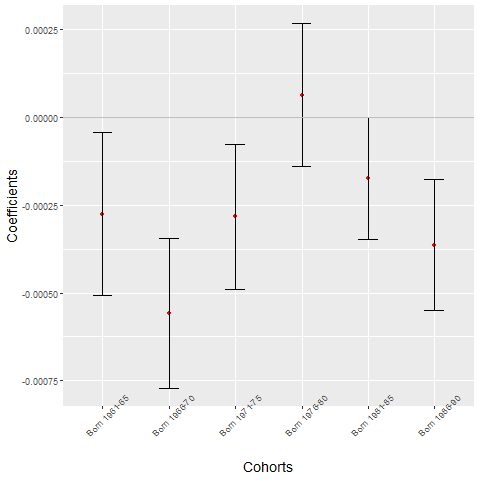
\includegraphics[scale = 0.6]{images/graph_coeff_pri_mig.png}
    \caption{$\hat{\beta}$'s estimated from \eqref{eq:lpm_yatra}, for completion of primary school after controlling for difference in Muslim population.}
    \label{fig:coeff_pri_mig}
\end{figure}

I provide corresponding estimates for illiteracy levels, secondary and college education in Figures \ref{fig:coeff_ill_mig}, \ref{fig:coeff_sec_mig}, and \ref{fig:coeff_col_mig}, respectively. I draw the same conclusions as above. 

\subsection{\textit{Yatra} and Scheduled Castes}
\cite{adukia.2018} and \cite{bharathi2018isolated} document caste-based residential segregation in various Indian cities. I check if the treatment affects education outcomes of Scheduled Castes differently, where this group is considered to be untreated. In Figure \ref{fig:li_pri_sc}, I observe parallel trends in SC and non-SC primary education attainment, with respect to distance from \textit{Yatra} route.  

\begin{figure}[H]
    \centering
    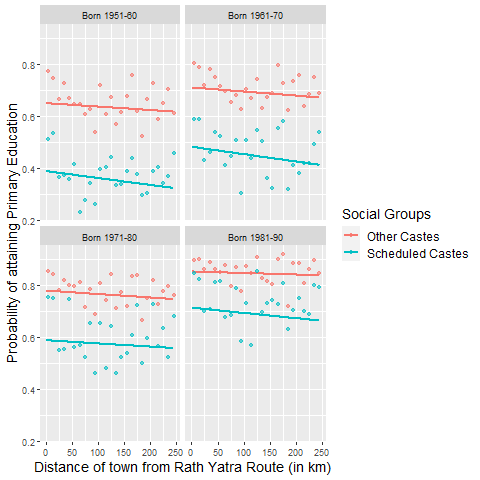
\includegraphics[scale = 0.7]{images/graph_li_pri_sc.png}
    \caption{Relationship between caste-based segregation measure (dissimilarity index for scheduled caster $\times$ 100) and distance from \textit{Yatra} route in kilometres.}
    \label{fig:li_pri_sc}
\end{figure}

Taken together, Figures \ref{fig:sc_disindex} and \ref{fig:li_pri_sc} provide evidence that segregation is the channel associated with better early education outcomes for Muslims in India.

\subsection{Non-Yatra States}
As a final placebo test, I check if the first stage relationship between distance from \textit{Yatra} route and dissimilarity index (measuring community/ religion based segregation) holds for states where the \textit{Ram Rath Yatra} campaign did not enter. In Figure \ref{fig:nonyatra_disindex}, I do not find statistically significant correlation between the treatment and segregation in these states. 

\begin{figure}[H]
    \centering
    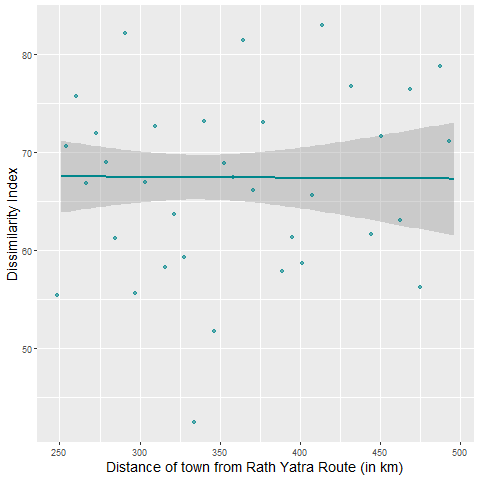
\includegraphics[scale = 0.6]{images/graph_nonyatra_disindex.png}
    \caption{Relationship between segregation measure (dissimilarity index $\times$ 100) and distance from \textit{Yatra} route in kilometres, for states that did not witness the \textit{Yatra} campaign.}
    \label{fig:nonyatra_disindex}
\end{figure}

Therefore, I do not find any spurious correlation in states that were not exposed to this campaign. I only consider cities within 250 to 500 kilometre range in these states, to avoid capturing spillovers to cities close to the \textit{Yatra} states. 

\section{Conclusion}\label{conclusion}
In this paper, I evaluated the long-term impacts of a violent event of great political significance in contemporary India. Surprisingly, I found that Muslims perform better in cities that were more susceptible to communal violence in terms of early education outcomes, whereas overall educational mobility of Muslims has been declining in the country.  I also found that cities that were closer to the route of the \textit{Ram Rath Yatra} are more segregated than cities farther away.

Based on the reduced form estimates, I isolated the causal impact of neighbourhood effects on Muslim education outcomes, using distance from \textit{Yatra} route as an instrument. I found that higher dissimilarity index leads to better early education outcomes for Muslims. I also demonstrated that the direction of the effect remains unchanged under less restrictive assumptions on the validity of the instrument.

I discuss various mechanisms through which neighbourhood effects could improve education outcomes. I stipulate that Muslim enclaves may witness \textit{stronger ties} within the community in the aftermath of communal violence. In this process, Muslims may not be forming \textit{weak ties} outside the community. This affects their ability to bargain for positions in higher education institutions. 

My findings open various avenues for future research. Firstly, it is worth enquiring how Muslim parents make schooling choice decisions for their children in cities, as we need a better understanding of school choice mechanisms in urban India. Secondly, the available data limits our understanding of inputs that produce quality education in urban schools. This has serious policy implications in Developing countries. 

Thirdly, I have only employed cross-sectional variation in segregation. Temporal variation in residential segregation would enable estimation of neighbourhood effects on education outcomes for various disadvantaged social groups. \cite{adukia.2018} also highlight that research employing better measures of residential segregation, than the one employed here, would also bring valuable insights. 

Finally, research backed by data on social networks, in segregated and integrated neighbourhoods, would provide a concrete understanding of the mechanisms through which the choice of residential neighbourhoods impacts educational outcomes of historically disadvantaged social groups. 

This paper contributes to existing literature on inter-group inequality in Developing countries by demonstrating the effect of communal violence on education outcomes of historically disadvantaged groups. I have also highlighted channels through which communal violence drives group education outcomes, and a deeper investigation into these mechanisms is a subject for future research. 

\newpage
\section*{References}
\bibliography{references.bib}

\newpage

\appendix
\section*{Appendix A: Graphs}\label{appendix_a}
\renewcommand\thefigure{A.\arabic{figure}}

\setcounter{figure}{0}
\begin{figure}[H]
    \centering
    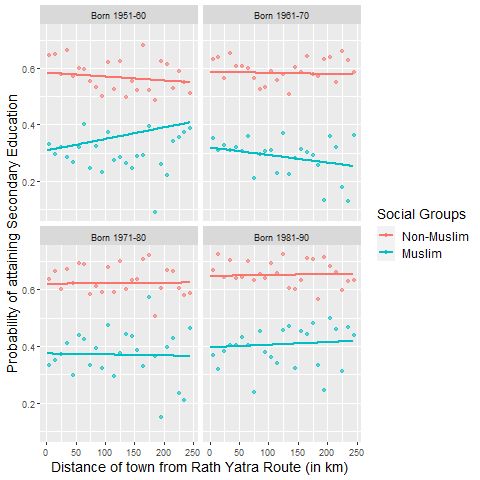
\includegraphics[scale = 0.7]{images/graph_li_sec_mus.png}
    \caption{Probability of attaining secondary education by religion, cohort, and distance from \textit{Yatra}}
    \label{fig:li_sec_mus} 
\end{figure}

\begin{figure}[H]
    \centering
    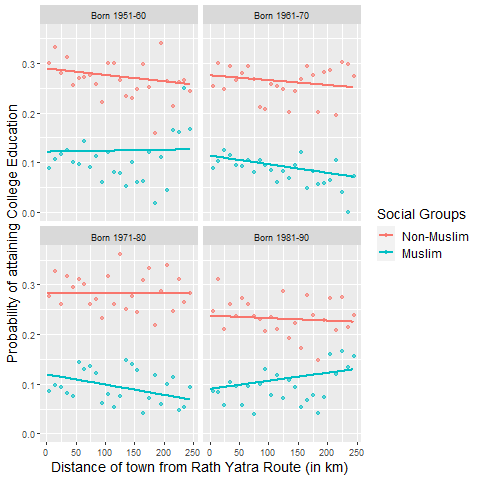
\includegraphics[scale = 0.7]{images/graph_li_col_mus.png}
    \caption{Probability of attaining college education by religion, cohort, and distance from \textit{Yatra}}
    \label{fig:li_col_mus}
\end{figure}

\begin{figure}[H]
    \centering
    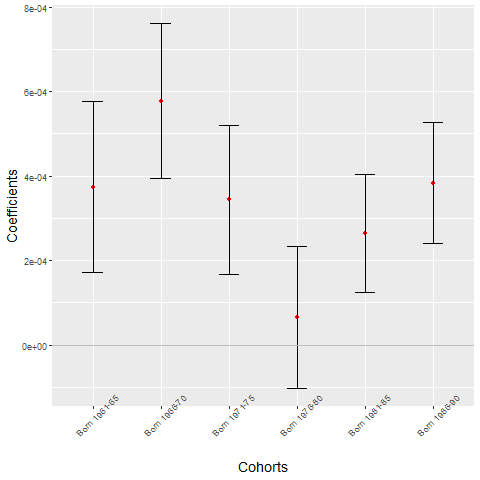
\includegraphics[scale = 0.5]{images/graph_coeff_ill.png}
    \caption{$\hat{\beta}$'s estimated from \eqref{eq:lpm_yatra}, for illiteracy levels}
    \label{fig:coeff_ill}
\end{figure}

\begin{figure}[H]
    \centering
    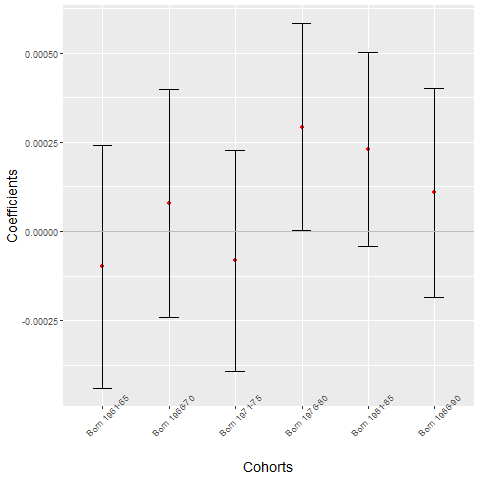
\includegraphics[scale = 0.5]{images/graph_coeff_sec.png}
    \caption{$\hat{\beta}$'s estimated from \eqref{eq:lpm_yatra}, for completion of secondary school}
    \label{fig:coeff_sec}
\end{figure}

\begin{figure}[H]
    \centering
    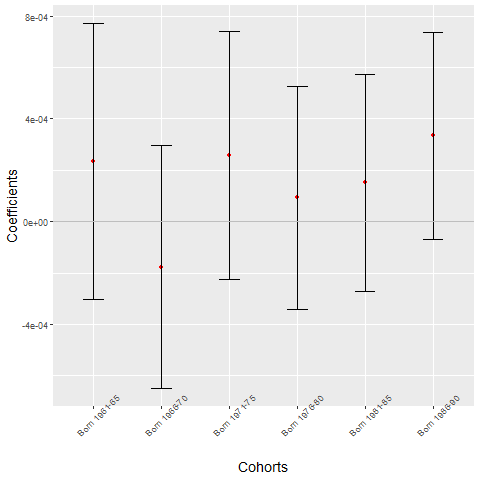
\includegraphics[scale = 0.5]{images/graph_coeff_col.png}
    \caption{$\hat{\beta}$'s estimated from \eqref{eq:lpm_yatra}, for attainment of college education}
    \label{fig:coeff_col}
\end{figure}

\begin{figure}[H]
    \centering
    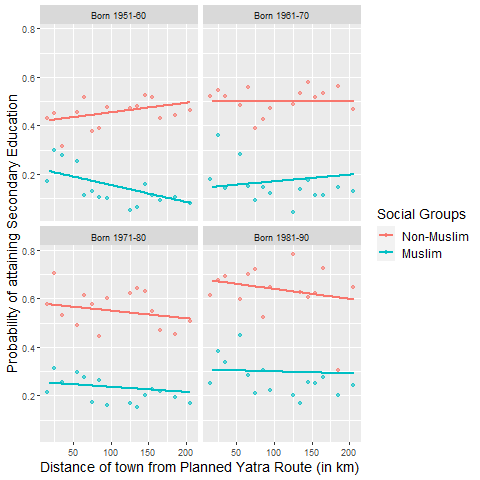
\includegraphics[scale = 0.7]{images/graph_li_sec_mus_p.png}
    \caption{Probability of attaining secondary education by religion, cohort, and distance from \textit{placebo Yatra}.}
    \label{fig:li_sec_mus_p}
\end{figure}

\begin{figure}[H]
    \centering
    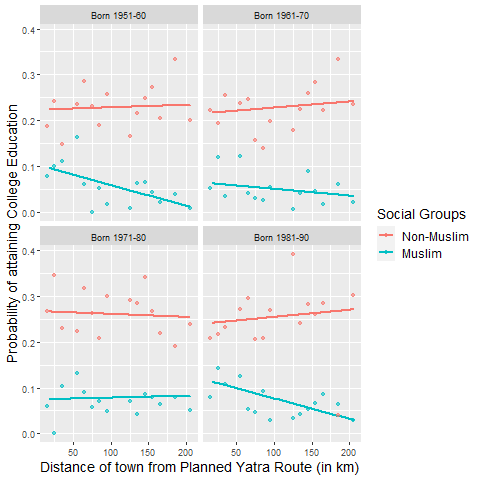
\includegraphics[scale = 0.7]{images/graph_li_col_mus_p.png}
    \caption{Probability of attaining college education by religion, cohort, and distance from \textit{placebo Yatra}.}
    \label{fig:li_col_mus_p}
\end{figure}

\begin{figure}[H]
    \centering
    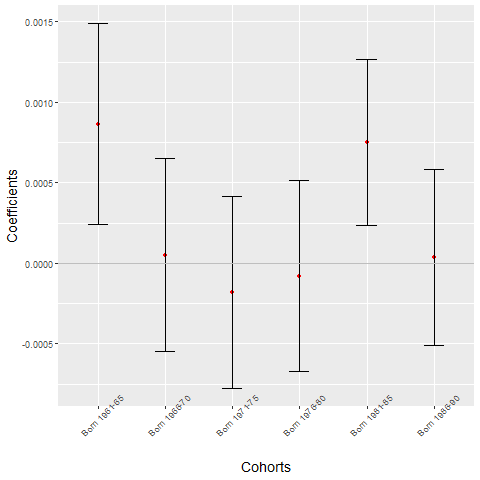
\includegraphics[scale = 0.4]{images/graph_coeff_ill_p.png}
    \caption{$\hat{\beta}$'s estimated from \eqref{eq:lpm_yatra_p} with respect to \textit{placebo Yatra}, for illiteracy levels}
    \label{fig:coeff_ill_p}
\end{figure}

\begin{figure}[H]
    \centering
    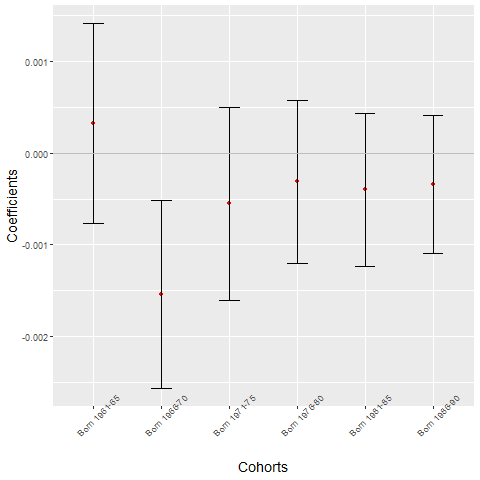
\includegraphics[scale = 0.4]{images/graph_coeff_sec_p.png}
    \caption{$\hat{\beta}$'s estimated from \eqref{eq:lpm_yatra_p} with respect to \textit{placebo Yatra}, for completion of secondary school.}
    \label{fig:coeff_sec_p}
\end{figure}

\begin{figure}[H]
    \centering
    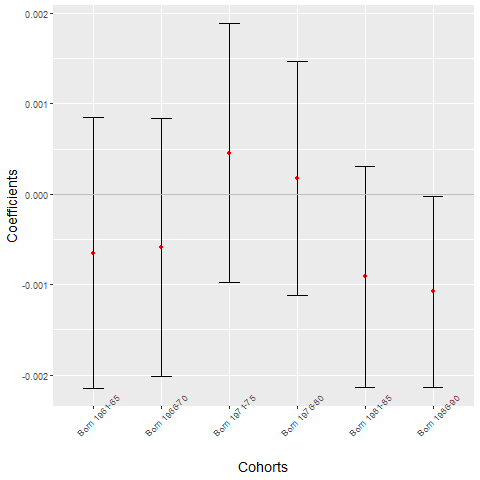
\includegraphics[scale = 0.4]{images/graph_coeff_col_p.png}
    \caption{$\hat{\beta}$'s estimated from \eqref{eq:lpm_yatra_p} with respect to \textit{placebo Yatra}, for completion of primary school.}
    \label{fig:coeff_col_p}
\end{figure}

\newpage
\begin{figure}[H]
    \centering
    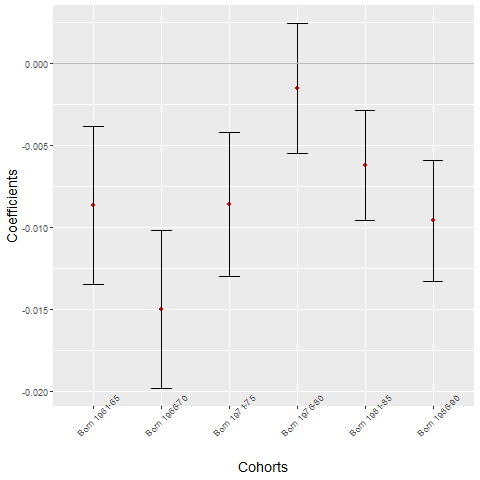
\includegraphics[scale = 0.5]{images/graph_coeff_ill_iv.png}
    \caption{IV estimates of $\hat{\beta}$'s from \eqref{eq:lpm_yatra_iv}, for illiteracy levels.}
    \label{fig:coeff_ill_iv}
\end{figure}

\begin{figure}[H]
    \centering
    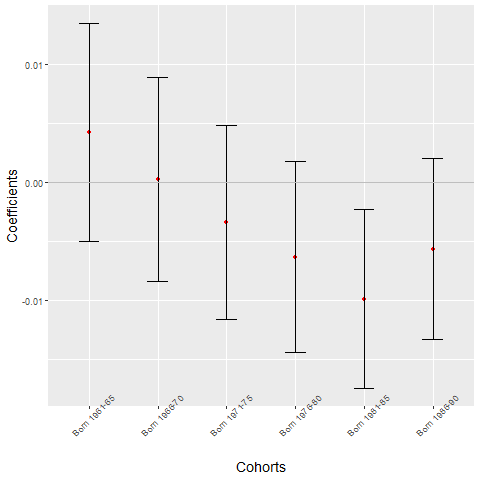
\includegraphics[scale = 0.5]{images/graph_coeff_sec_iv.png}
    \caption{IV estimates of $\hat{\beta}$'s from \eqref{eq:lpm_yatra_iv}, for completion of secondary school.}
    \label{fig:coeff_sec_iv}
\end{figure}

\begin{figure}[H]
    \centering
    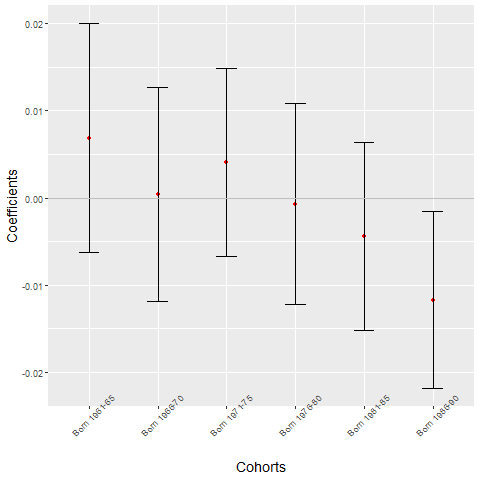
\includegraphics[scale = 0.5]{images/graph_coeff_col_iv.png}
    \caption{IV estimates of $\hat{\beta}$'s from \eqref{eq:lpm_yatra_iv}, for completion of college}
    \label{fig:coeff_col_iv}
\end{figure}

\begin{figure}[H]
    \centering
    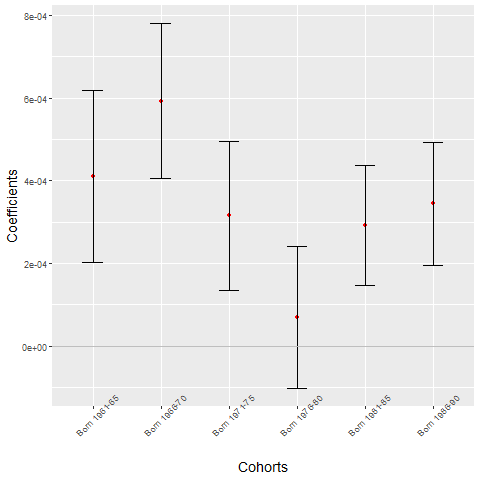
\includegraphics[scale = 0.4]{images/graph_coeff_ill_mig.png}
    \caption{$\hat{\beta}$'s estimated from \eqref{eq:lpm_yatra}, for illiteracy levels after controlling for difference in Muslim population.}
    \label{fig:coeff_ill_mig}
\end{figure}

\begin{figure}[H]
    \centering
    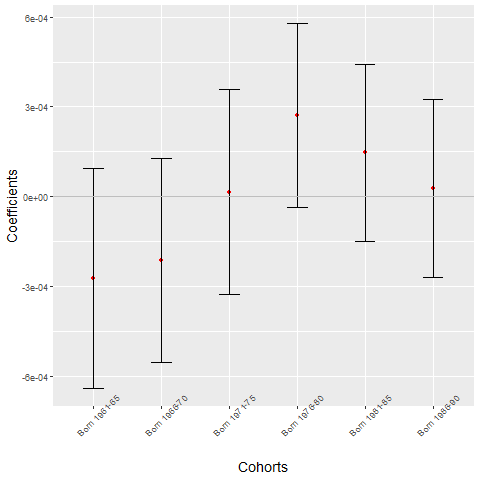
\includegraphics[scale = 0.4]{images/graph_coeff_sec_mig.png}
    \caption{$\hat{\beta}$'s estimated from \eqref{eq:lpm_yatra}, for completion of secondary school after controlling for difference in Muslim population.}
    \label{fig:coeff_sec_mig}
\end{figure}

\begin{figure}[H]
    \centering
    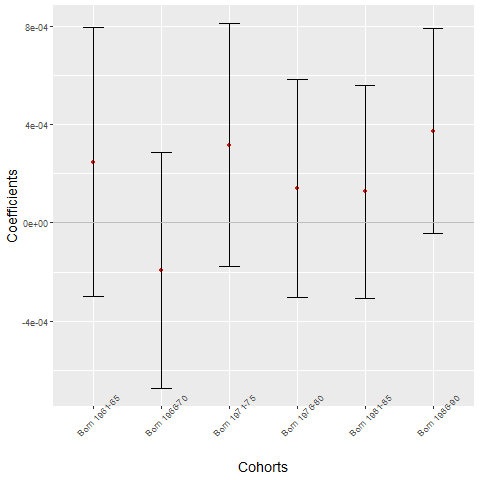
\includegraphics[scale = 0.4]{images/graph_coeff_col_mig.png}
    \caption{$\hat{\beta}$'s estimated from \eqref{eq:lpm_yatra}, for college education after controlling for difference in Muslim population.}
    \label{fig:coeff_col_mig}
\end{figure}

\newpage
\section*{Appendix B: Tables}\label{appendix_b}
\renewcommand\thetable{B.\arabic{table}}

\setcounter{table}{0}

\begin{table}[H]
    \resizebox{\textwidth}{!}{
    \centering
    {
\def\sym#1{\ifmmode^{#1}\else\(^{#1}\)\fi}
\begin{tabular}{l*{7}{c}}
\hline\hline
            &\multicolumn{1}{c}{(1)}&\multicolumn{1}{c}{(2)}&\multicolumn{1}{c}{(3)}&\multicolumn{1}{c}{(4)}&\multicolumn{1}{c}{(5)}&\multicolumn{1}{c}{(6)}&\multicolumn{1}{c}{(7)}\\
 Born           &\multicolumn{1}{c}{Before 1951}&\multicolumn{1}{c}{1951-55}&\multicolumn{1}{c}{1956-60}&\multicolumn{1}{c}{1961-65}&\multicolumn{1}{c}{1966-70}&\multicolumn{1}{c}{1971-75}&\multicolumn{1}{c}{1976-80}\\
 [1em]
\hline
\textbf{Illiteracy Level} & & \\
[1em]
\textit{Yatra} distance $\times$ Muslim &    0.000129 &    -0.00000257 & 0.000224 & 0.000291\sym{**} & 0.000386\sym{***} & 0.000214\sym{*} &   0.0000971\\
            &  (0.000102)         & (0.000137)    & (0.000127) & (0.000111) & (0.0000990) & (0.0000979) & (0.0000888)  \\
[1em]
\hline
\textbf{Primary School} & & \\
[1em]
&  -0.0000594 &  0.000121 &   -0.000231 & -0.000262\sym{*} &   -0.000338\sym{***} & -0.000161 &  -0.0000550\\
& (0.000107)         & (0.000142) &  (0.000131)   &  (0.000114)   &  (0.000102) &  (0.000100) & (0.0000908)\\
[1em]
\hline
\textbf{Secondary School} & & \\
[1em]
&    0.000353 &    0.000231    &    0.000296    & -0.000376 & -0.000132 &    0.000174 &    0.000316\\
&  (0.000181)         &  (0.000249)  &  (0.000238)  &  (0.000203) &  (0.000202)  &  (0.000204) &  (0.000183) \\
[1em]
\hline
\textbf{College} & & \\
[1em]
&    -0.000124 &    -0.000398 & 0.000900\sym{**} & -0.000485 &  -0.0000928 & -0.000307 & 0.0000384\\
&  (0.000265) &  (0.000354) & (0.000344) &  (0.000305) &  (0.000294) &  (0.000268) & (0.000248)\\
[1em]
\hline\hline
\multicolumn{3}{l}{\footnotesize Standard errors in parentheses}\\
\multicolumn{3}{l}{\footnotesize \sym{*} \(p<0.05\), \sym{**} \(p<0.01\), \sym{***} \(p<0.001\)}\\
\end{tabular}
}
    }
    \caption{Relationship between distance from \textit{Yatra} route (in km) and education attainment levels for Muslims born after 1980, weighted by stabilized IPW.}
    \label{tab:education_score_re_old}
\end{table}

\newpage
\section*{Section C: Concepts and Definitions}

\subsection*{Dissimilarity Index}

Residential segregation, for some city $c$, is measured with the Dissimilarity Index \citep{massey.2018}:

\begin{equation}\label{eq:dis_index}
d_c = \frac{1}{2} \sum_i \Bigl|\frac{m_{ic}}{M_c} - \frac{h_{ic}}{H_c}\Bigr|
\end{equation}

where, $m_{ic}$ is the Muslim population in city $c$ in EB $i$, $M_c$ is the total population of Muslims in city $c$, $h_{ic}$ is the non-Muslim population in city $c$ in EB $i$, and $H_c$ is the total population of non-Muslims in city $c$.

Essentially, the dissimilarity index captures evenness in the distribution of the two social groups across neighbourhoods that constitute a city. Its value ranges between 0 and 1, where the value of $d_c$ attains the maximum value when each neighbourhood has residents from only one group. On the other hand $d_c$ is at its miniumum when $\frac{m_{ic} / T_c}{M_c / T_c} = \frac{h_{ic} / T_c}{H_c / T_c}$ in all neighbourhoods $i$ in city $c$ where $T_c$ is the total population in the city. In other words, $d_c = 0$ when  proportion of each group in each neighbourhood equals the proportion of each group in the city, i.e. 
$$\frac{m_{ic} / T_c}{h_{ic} / T_c} = \frac{M_c / T_c}{H_c / T_c}$$

\end{document}
